\documentclass[12pt,a4paper]{article}
 
\usepackage{float}
%für feststellen der figures und tables [H] dranschreiben
\usepackage{units}
%wird so benutzt: 
%\unit[value/Zahl]{dimension/Einheit} oder 
%\unitfrac[value/Zahl]{dimension/Einheit num/Zähler}{dimension/Einheit denum/Nenner} oder
%\nicefrac[fontcommand/Schriftart]{dimension/Einheit num/Zähler}{dimension/Einheit denum/Nenner}

\usepackage{caption}
\usepackage{subcaption}

\usepackage[left=2cm,right=2cm,top=2cm,bottom=2cm]{geometry}
\usepackage[utf8]{inputenc}
\usepackage[T1]{fontenc}
\usepackage{lmodern}
\usepackage[ngerman]{babel}
\usepackage{amsmath}
\usepackage{graphicx}
 
\title{Versuch ...\\}
\author{Frederik Strothmann, Henrik Jürgens}
\date{\today}
%niemals zwei überschriften direkt übereinander schreiben, also immer mindestens in einem satz was sinnvolles unter jede überschrift schreiben (bei den versuchen z.B. das versuchsziel) 
\begin{document}
%deckblatt erstellen.
\maketitle
\newpage
\tableofcontents
\newpage
\section{Einleitung}
%einleitung zu dem experiment.
%auf die einstellungen, die vor dem versuch gemacht werden, eingehen oder auf eine anleitung dazu verweisen
%es soll immer erwähnt werden um was es in dem Versuch geht und wie das relisiert werden soll
%---------------------------------------------------------------------------------------------
%hinter der einleitung kann der allgemeine theoretische hintergrund in einer zusätzlichen section erklärt werden
%1-----------------------------------------------1

\section{Simulation mit passiver Bauelementen}

In diesem Versuchsabschnitt werden verschiedene Schaltungen aus passiven Bauelementen auf ihre Eigenschaften untersucht.

\subsection{Auf- und Entladekurve eines RC-Kreises}
%kurz das ziel dieses versuchsteiles ansprechen, damit keine zwei überschriften direkt übereinander stehen!
%bei schwierigeren versuchen kann auch der theoretische hintergrund erläutert werden. (mit formeln, herleitungen und erklärungen)

In diesem Versuchsteil soll ein RC-Kreis simuliert werden und dabei die Auf- und Entladekurve aufgenommen werden.

\subsubsection{Verwendete Geräte}
%(immer) eine skizze oder ein foto einfügen, die geräte/materialien !nummerieren! und z.b. eine legende dazu schreiben, besser wäre es das ganze in einem Fließtext gut zu beschreiben.
%falls am anfang des versuches nicht klar ist, was alles verwendet wird, wenn möglich erst am ende ein großes foto von den verwendeten materialien machen!\\

Es werden ein Funktionsgenerator, ein Widerstand, ein Kondensator und ein Oszillator verwendet.

\subsubsection{Verwendete Formeln}
%eine legende kann angefertigt werden, die selbstverständlichen buchstaben müssen nicht extra erklärt werden
%mit knappen erklärungen die !verwendeten! formeln, sowie die zugehörige fehlerrechnung einfügen
%2-----------------------------------------------2
%ab hier kann nochmal in einzelne versuchsteile unterteilt werden

Die Halbwertszeit $\tau$ ergibt sich aus der Gleichung:

\begin{align}
\tau = \text{ln}(2) \cdot \text{R} \cdot \text{C}
\label{eqn:tau}
\end{align}

\subsubsection{Versuchsaufbau}
%skizze zum versuchsaufbau (oder foto) einfügen,   es muss erklärt werden wie das ganze funktioniert und welche speziellen einstellungen verwendet wurden (z.b. welche knöpfe an den geräten für die messung verdreht wurden)

R1 ist ein 1k$\Omega$ Widerstand und C1 ein 1$\mu$F Kondensator.

\begin{figure}[H] 
  \centering
    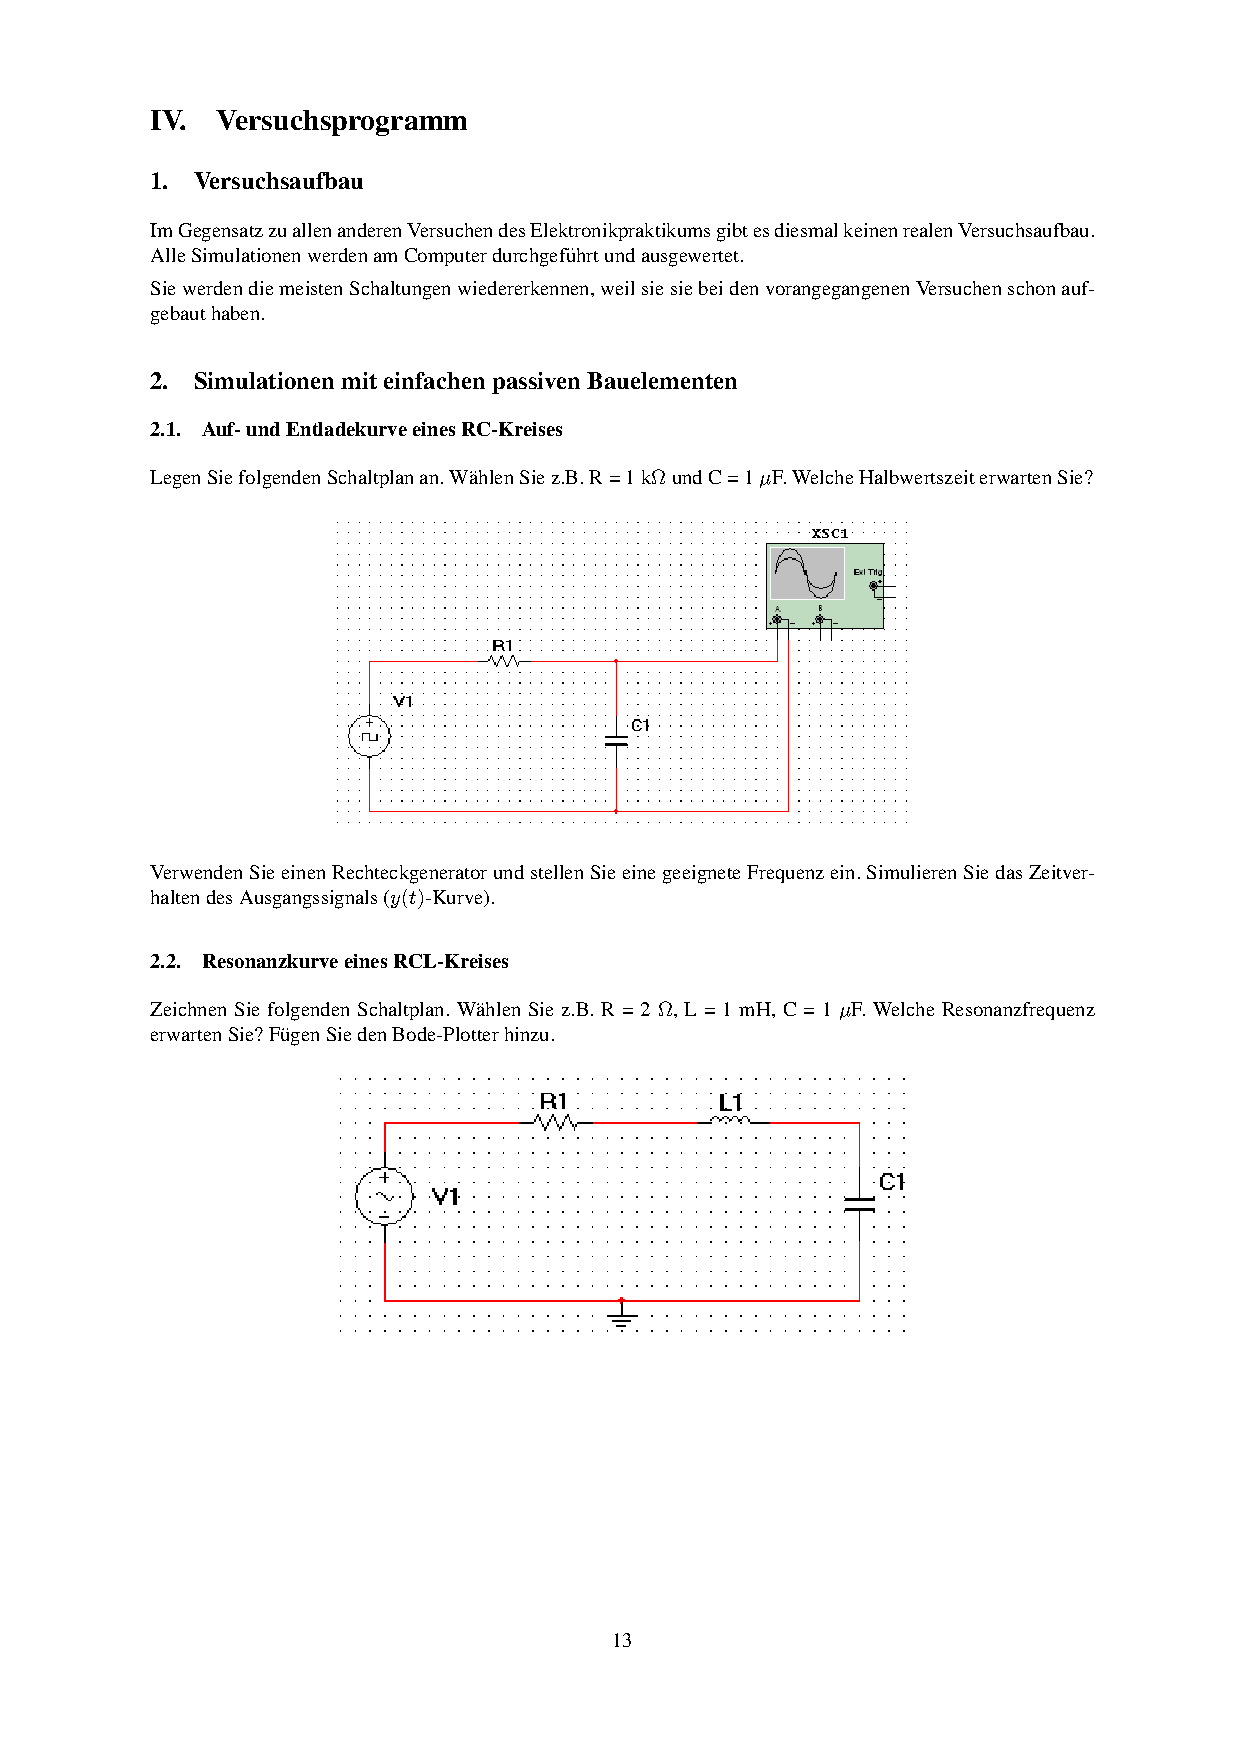
\includegraphics[trim = 10mm 155mm 10mm 85mm, clip, scale = 1]{ep5_14[Page13].pdf}
  	\caption[Schaltskizze des RC-Kreises]{Schaltskizze des RC-Kreises\footnotemark}
  \label{fig:1_a_1}
\end{figure}
\footnotetext{Abbildung entnommen von http://www.atlas.uni-wuppertal.de/$\sim$kind/ep5\_14.pdf Seite 13 am 22.11.2014}

\subsubsection{Versuchsdurchführung}
%erklären, !was! wir machen, !warum! wir das machen und mit welchem ziel
%(wichtig) präzize erklären, wie bei dem versuch vorgegangen und was gemacht wurde


Zuerst wird die Schaltung nach Abbildung \ref{fig:1_a_1} aufgebaut. Es wird das Fenster des Oszilloskops aufgerufen und die Simulation gestartet. Da die Kurve auf der y-Achse von 0 aus läuft kann mit einem Taster der maximal Wert bestimmt werden und  dann mit beiden Tastern die Halbwertszeit.


\subsubsection{Auswertung}
%zuerst !alle! errechneten werte entweder in ganzen sätzen aufzählen, oder in tabellen (übersichtlicher) dargestellen, sowie auf die verwendeten formeln verweisen (die referenzierung der formel kann in der überschrift stehen)
%kurz erwähnen (vor der tabelle), warum wir das ganze ausrechnen bzw. was wir dort ausrechnen
%danach histogramme und plots erstellen, wobei wenn möglich funktionen durch die plots gelegt werden (zur not können auch splines benutzt werden, was aber angegeben werden muss)
%bei fits immer die funktion und das reduzierte chiquadrat mit angegeben, wobei auf verständlichkeit beim entziffern der zehnerpotenzen geachtet werden muss z.b. f(x)=(wert+-fehler)\cdot10^{irgendeine zahl}\cdot x + (wert+-fehler)\cdot10^{irgendeine zahl}
%bei jedem fit erklären, nach welchem zusammenhang gefittet wurde und warum!
%bei plots darauf achten, dass die achsenbeschriftung (auch die tics) die richtige größe haben und die legende im plot nicht die messwerte verdeckt
%kurz die aufgabenstellung abhandeln
%2-----------------------------------------------2

Aus der theoretischen Berechnung ergibt sich eine theoretische Halbwertszeit von 1ms, siehe Gleichung \ref{eqn:tau}. Gemessen wurde eine Halbwertszeit von 0,693ms, wie in Abbildung \ref{fig:2_1} zu sehen ist.

\begin{figure}[H] 
  \centering
    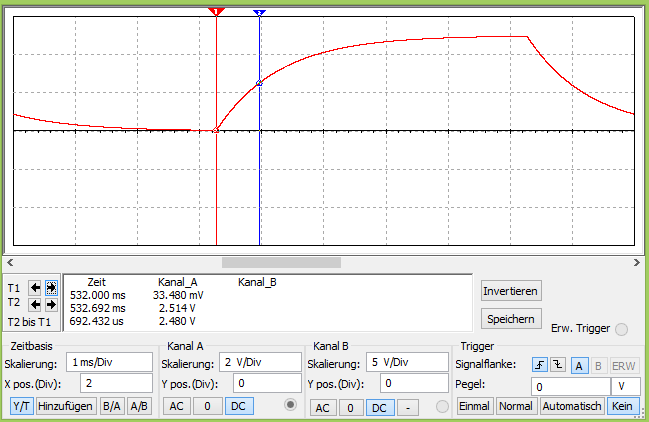
\includegraphics[ scale = 0.7]{2_1.PNG}
  	\caption[Auf- und Entladekurve des RC-Kreises]{Auf- und Entladekurve des RC-Kreises}
  \label{fig:2_1}
\end{figure}

\subsubsection{Diskussion}
%(immer) die gemessenen werte und die bestimmten werte über die messfehler mit literaturwerten oder untereinander vergleichen
%in welchem fehlerintervall des messwertes liegt der literaturwert oder der vergleichswert?
%wie ist der relative anteil des fehlers am messwert und damit die qualität unserer messung?
%in einem satz erklären, wie gut unser fehler und damit unsere messung ist
%kurz erläutern, wie systematische fehler unsere messung beeinflusst haben könnten
%(wichtig) zum schluss ansprechen, in wie weit die ergebnisse mit der theoretischen vorhersage übereinstimmen
%--------------------------------------------------------------------------------------------
%falls tabellen mit den messwerten zu lang werden, kann die section mit den messwerten auch hinter der diskussion angefügt bzw. eine section mit dem anhang eingefügt werden.
%1-----------------------------------------------1

Bei der Bestimmung der Halbwertszeit mit Multisim ergab sich eine etwas geringere Halbwertszeit als theoretisch vorhergesagt.

\subsection{Resonanzkurve eines RCL-Kreises}
%kurz das ziel dieses versuchsteiles ansprechen, damit keine zwei überschriften direkt übereinander stehen!
%bei schwierigeren versuchen kann auch der theoretische hintergrund erläutert werden. (mit formeln, herleitungen und erklärungen)

In diesem Versuchsteil soll ein RCL-Kreis auf seine Resonanzfrequenz untersucht werden. Für die Untersuchung mit Multisim wir ein Bode-Plot verwendet.

\subsubsection{Verwendete Geräte}
%(immer) eine skizze oder ein foto einfügen, die geräte/materialien !nummerieren! und z.b. eine legende dazu schreiben, besser wäre es das ganze in einem Fließtext gut zu beschreiben.
%falls am anfang des versuches nicht klar ist, was alles verwendet wird, wenn möglich erst am ende ein großes foto von den verwendeten materialien machen!\\

Es werden ein Funktionsgenerator, ein Widerstand, ein Kondensator und eine Spule verwendet.

\subsubsection{Verwendete Formeln}
%eine legende kann angefertigt werden, die selbstverständlichen buchstaben müssen nicht extra erklärt werden
%mit knappen erklärungen die !verwendeten! formeln, sowie die zugehörige fehlerrechnung einfügen
%2-----------------------------------------------2
%ab hier kann nochmal in einzelne versuchsteile unterteilt werden

Theoretisch ergibt sich die Resonanzfrequenz eines RCL-Kreises aus der Gleichung:

\begin{align}
\text{f}_0 = \frac{1}{2 \pi \sqrt{\text{RL}}}
\label{eqn:f0}
\end{align}

\subsubsection{Versuchsaufbau}
%skizze zum versuchsaufbau (oder foto) einfügen,   es muss erklärt werden wie das ganze funktioniert und welche speziellen einstellungen verwendet wurden (z.b. welche knöpfe an den geräten für die messung verdreht wurden)

R1 ist ein 2$\Omega$ Widerstand, C1 ein 1$\mu$F Kondensator und L1 eine 1mH Spule.

\begin{figure}[H] 
  \centering
    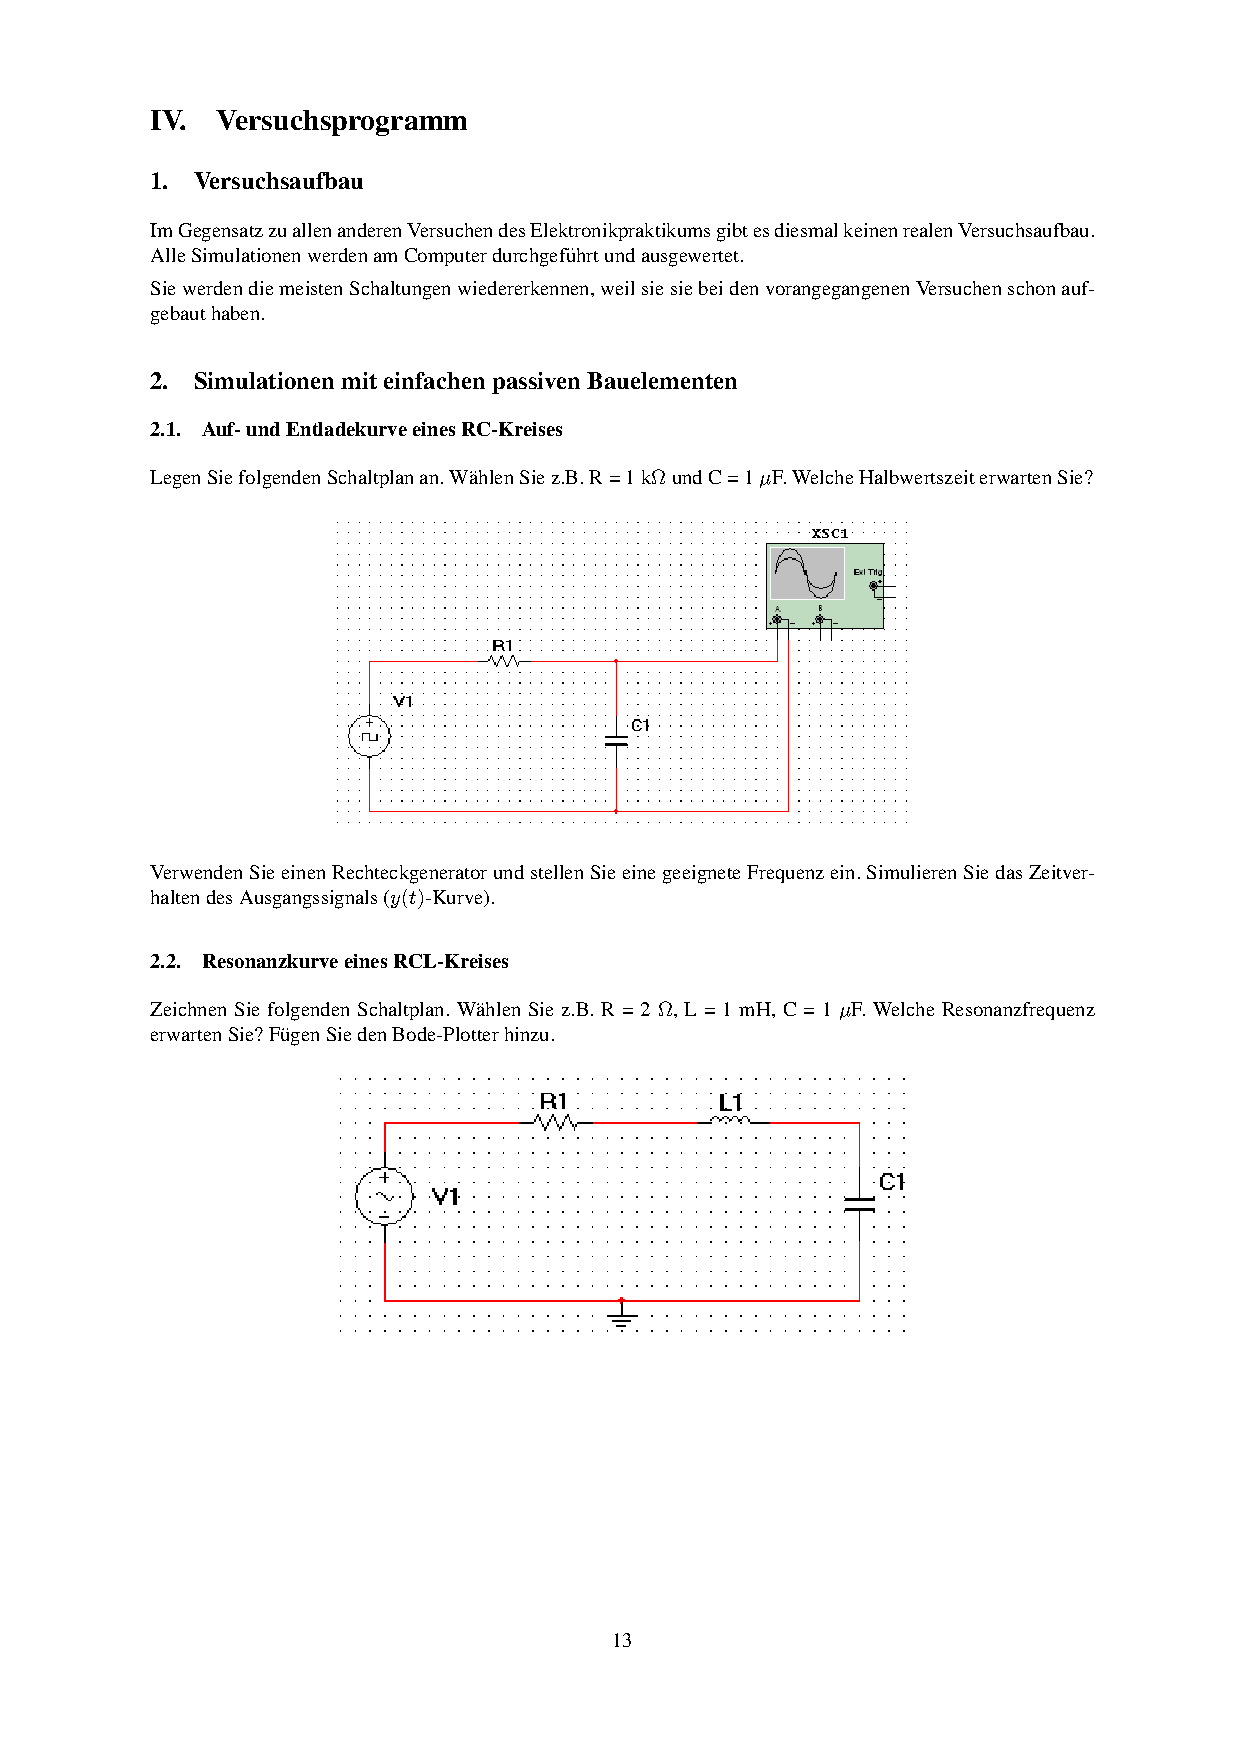
\includegraphics[trim = 10mm 60mm 10mm 178mm, clip, scale = 1]{ep5_14[Page13].pdf}
  	\caption[Schaltskizze des RCL-Kreises]{Schaltskizze des RCL-Kreises\footnotemark}
  \label{fig:1_a_2}
\end{figure}
\footnotetext{Abbildung entnommen von http://www.atlas.uni-wuppertal.de/$\sim$kind/ep5\_14.pdf Seite 13 am 22.11.2014}

\subsubsection{Versuchsdurchführung}
%erklären, !was! wir machen, !warum! wir das machen und mit welchem ziel
%(wichtig) präzize erklären, wie bei dem versuch vorgegangen und was gemacht wurde

Zu erst wird die Schaltung nach Abbildung \ref{fig:1_a_2} aufgebaut und der Bodeplotter angeschlossen. Es wird das Fenster des Bodeplotters aufgerufen und der Frequenzbereich so wie der Dezibel-Bereich eingestellt. Dabei sollte darauf geachtet werden, dass man den Frequenzbereich möglichst nah um die Resonanzfrequenz wählt. Dann wird die Simulation gestartet und die Resonanzfrequenz mit dem Taster bestimmt.


\subsubsection{Auswertung}
%zuerst !alle! errechneten werte entweder in ganzen sätzen aufzählen, oder in tabellen (übersichtlicher) dargestellen, sowie auf die verwendeten formeln verweisen (die referenzierung der formel kann in der überschrift stehen)
%kurz erwähnen (vor der tabelle), warum wir das ganze ausrechnen bzw. was wir dort ausrechnen
%danach histogramme und plots erstellen, wobei wenn möglich funktionen durch die plots gelegt werden (zur not können auch splines benutzt werden, was aber angegeben werden muss)
%bei fits immer die funktion und das reduzierte chiquadrat mit angegeben, wobei auf verständlichkeit beim entziffern der zehnerpotenzen geachtet werden muss z.b. f(x)=(wert+-fehler)\cdot10^{irgendeine zahl}\cdot x + (wert+-fehler)\cdot10^{irgendeine zahl}
%bei jedem fit erklären, nach welchem zusammenhang gefittet wurde und warum!
%bei plots darauf achten, dass die achsenbeschriftung (auch die tics) die richtige größe haben und die legende im plot nicht die messwerte verdeckt
%kurz die aufgabenstellung abhandeln
%2-----------------------------------------------2

Aus Gleichung \ref{eqn:f0} ergibt sich eine erwartete Resonanzfrequenz von \unit[5,033]{kHz}, gemessen wurde eine Resonanzfrequenz von \unit[5,011]{kHz}, siehe Abbildung \ref{fig:2_2}.

\begin{figure}[H] 
  \centering
    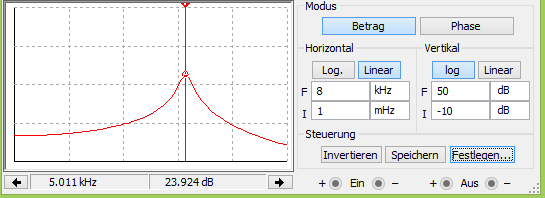
\includegraphics[ scale = 0.7]{2_2_resonanz.PNG}
  	\caption[Bodeplot des RCL-Kreises]{Bodeplot des RCL-Kreises}
  \label{fig:2_2}
\end{figure}


\subsubsection{Diskussion}
%(immer) die gemessenen werte und die bestimmten werte über die messfehler mit literaturwerten oder untereinander vergleichen
%in welchem fehlerintervall des messwertes liegt der literaturwert oder der vergleichswert?
%wie ist der relative anteil des fehlers am messwert und damit die qualität unserer messung?
%in einem satz erklären, wie gut unser fehler und damit unsere messung ist
%kurz erläutern, wie systematische fehler unsere messung beeinflusst haben könnten
%(wichtig) zum schluss ansprechen, in wie weit die ergebnisse mit der theoretischen vorhersage übereinstimmen
%--------------------------------------------------------------------------------------------
%falls tabellen mit den messwerten zu lang werden, kann die section mit den messwerten auch hinter der diskussion angefügt bzw. eine section mit dem anhang eingefügt werden.
%1-----------------------------------------------1

Die mit Multisim bestimmte Resonanzfrequenz liegt sehr nah bei der erwarteten Resonanzfrequenz, was zu erwarten war.


\subsection{Rechtecksignal am RCL-Kreises}
%kurz das ziel dieses versuchsteiles ansprechen, damit keine zwei überschriften direkt übereinander stehen!
%bei schwierigeren versuchen kann auch der theoretische hintergrund erläutert werden. (mit formeln, herleitungen und erklärungen)

In diesem Versuchsteil soll der Effekt des Widerstandes R im RCL-Kreis untersucht werden.

\subsubsection{Verwendete Geräte}
%(immer) eine skizze oder ein foto einfügen, die geräte/materialien !nummerieren! und z.b. eine legende dazu schreiben, besser wäre es das ganze in einem Fließtext gut zu beschreiben.
%falls am anfang des versuches nicht klar ist, was alles verwendet wird, wenn möglich erst am ende ein großes foto von den verwendeten materialien machen!\\

Es werden ein Funktionsgenerator, ein Widerstand, ein Kondensator, eine Spule und ein Oszilloskop verwendet.

\subsubsection{Versuchsaufbau}
%skizze zum versuchsaufbau (oder foto) einfügen,   es muss erklärt werden wie das ganze funktioniert und welche speziellen einstellungen verwendet wurden (z.b. welche knöpfe an den geräten für die messung verdreht wurden)

R1 ist ein 50$\Omega$ Widerstand, C1 ein 100nF Kondensator und L1 eine 1,5mH Spule. Der Frequenzgenerator wird mit einer Frequenz von 1kHz betrieben.

\begin{figure}[H] 
  \centering
    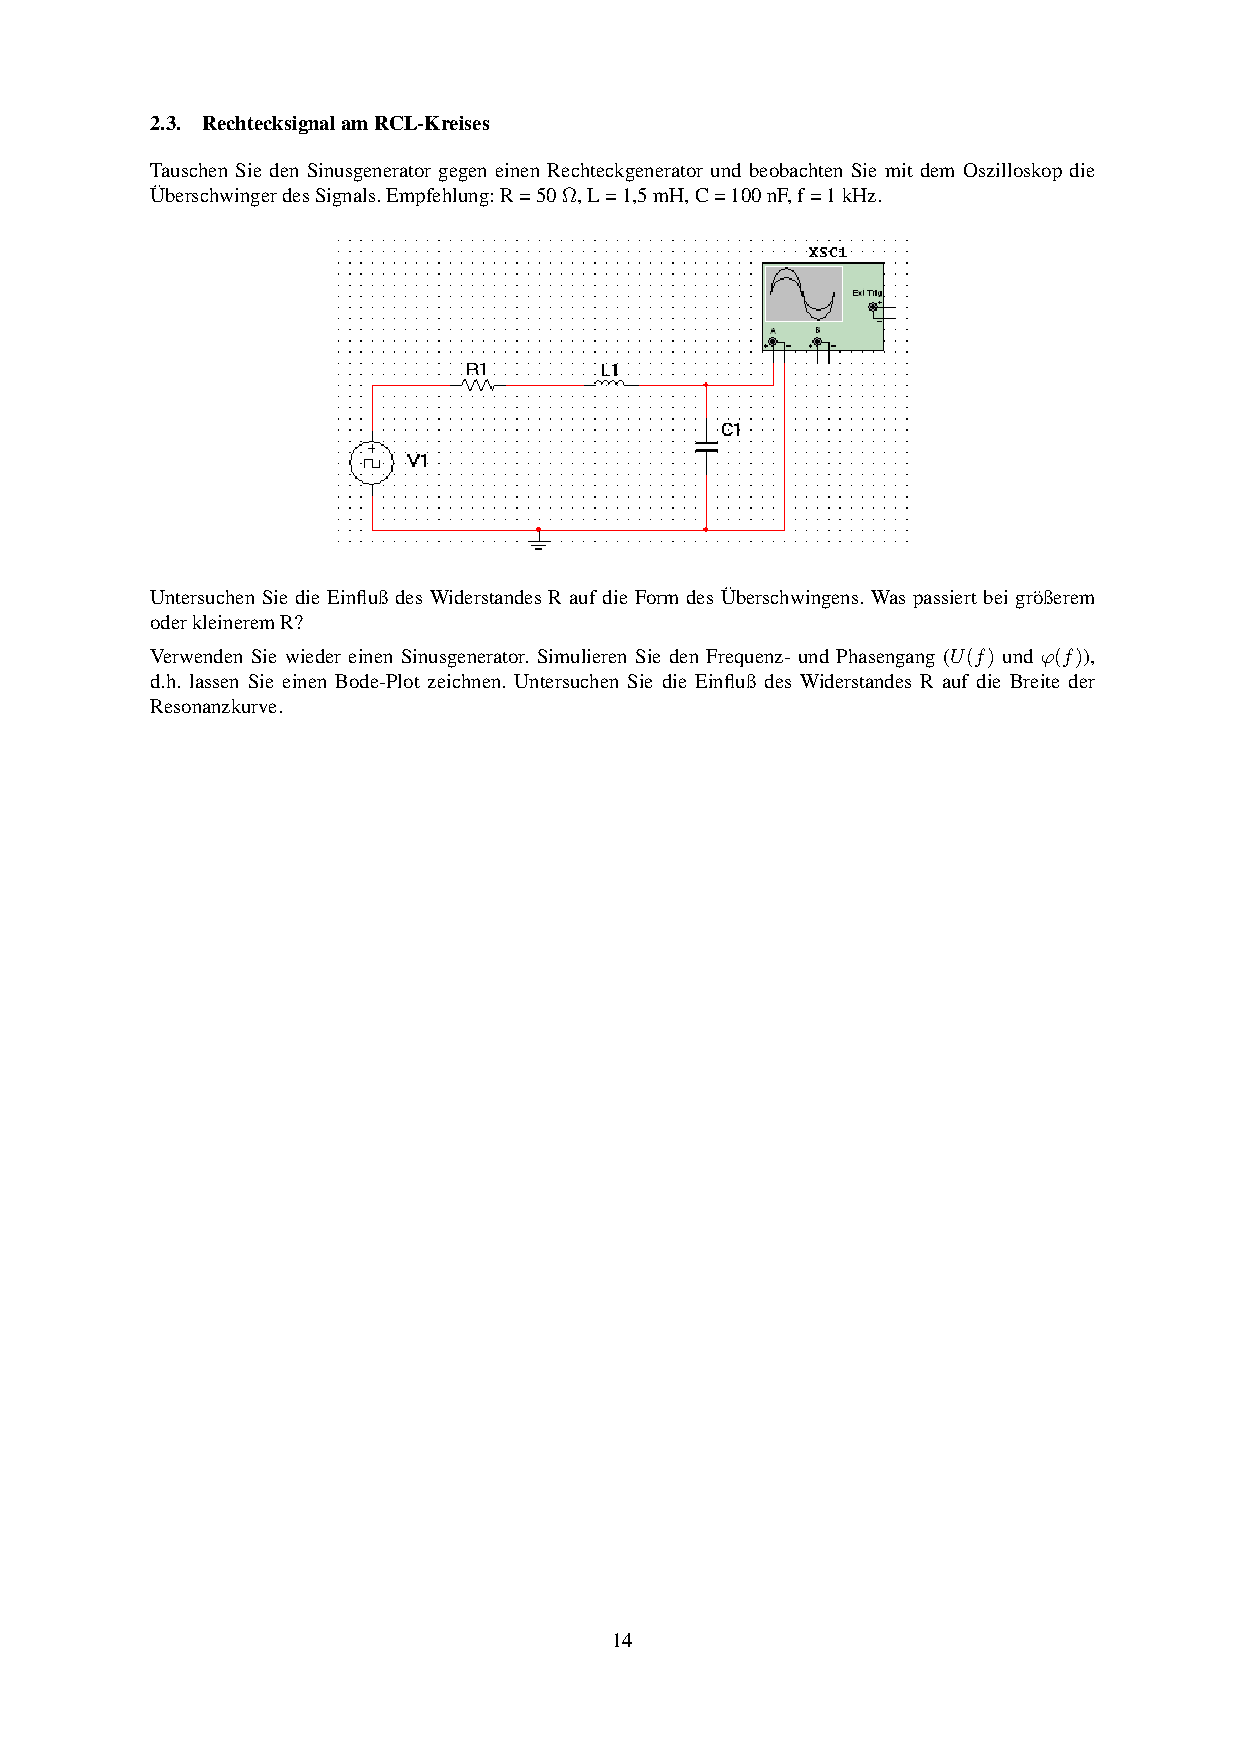
\includegraphics[trim = 10mm 200mm 10mm 40mm, clip, scale = 1]{ep5_14[Page14].pdf}
  	\caption[Schaltskizze des RCL-Kreises]{Schaltskizze des RCL-Kreises\footnotemark}
  \label{fig:1_a_3}
\end{figure}
\footnotetext{Abbildung entnommen von http://www.atlas.uni-wuppertal.de/$\sim$kind/ep5\_14.pdf Seite 14 am 22.11.2014}

\subsubsection{Versuchsdurchführung}
%erklären, !was! wir machen, !warum! wir das machen und mit welchem ziel
%(wichtig) präzize erklären, wie bei dem versuch vorgegangen und was gemacht wurde

Die Schaltung wird nach Abbildung \ref{fig:1_a_3} aufgebaut. Zu erst sollte der Effekt des Widerstandes auf die Überschwinger der Rechteckspannung untersucht werden, dafür wurde der Widerstand eingestellt (\unit[50]{$\Omega$},\unit[150]{$\Omega$} und \unit[300]{$\Omega$}), das Fenster des Oszilloskops aufgerufen und die Simulation gestartet. Im zweitem Teil sollte untersucht werden, wie sich R auf die Breite der Resonanzkurve auswirkt, dabei werden für R Werte von \unit[25]{$\Omega$} und \unit[50]{$\Omega$} verwendet. Dafür wurde R eingestellt, das Fenster des Bodeplotters aufgerufen und dann die Simulation gestartet.


\subsubsection{Auswertung}
%zuerst !alle! errechneten werte entweder in ganzen sätzen aufzählen, oder in tabellen (übersichtlicher) dargestellen, sowie auf die verwendeten formeln verweisen (die referenzierung der formel kann in der überschrift stehen)
%kurz erwähnen (vor der tabelle), warum wir das ganze ausrechnen bzw. was wir dort ausrechnen
%danach histogramme und plots erstellen, wobei wenn möglich funktionen durch die plots gelegt werden (zur not können auch splines benutzt werden, was aber angegeben werden muss)
%bei fits immer die funktion und das reduzierte chiquadrat mit angegeben, wobei auf verständlichkeit beim entziffern der zehnerpotenzen geachtet werden muss z.b. f(x)=(wert+-fehler)\cdot10^{irgendeine zahl}\cdot x + (wert+-fehler)\cdot10^{irgendeine zahl}
%bei jedem fit erklären, nach welchem zusammenhang gefittet wurde und warum!
%bei plots darauf achten, dass die achsenbeschriftung (auch die tics) die richtige größe haben und die legende im plot nicht die messwerte verdeckt
%kurz die aufgabenstellung abhandeln
%2-----------------------------------------------2

Bei der Untersuchung der Wirkung von R auf die Überschwinger der Rechteckspannung wurden drei Aufnahmen gemacht, bei \unit[50]{$\Omega$}, \unit[150]{$\Omega$} und \unit[300]{$\Omega$}. Dabei ergaben sich die Kurven in Abbildung \ref{fig:2_3_1}. Es ist deutlich zu sehen, dass ab \unit[150]{$\Omega$} die Überschwinger fast raus geblockt sind.


\begin{figure}[H]
        \centering
        \begin{subfigure}[b]{0.28\textwidth}
                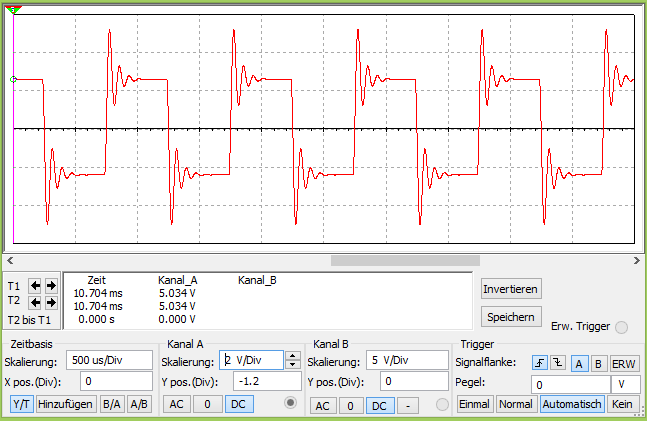
\includegraphics[width=\textwidth , scale = 0.4]{2_3_widerstand_50Ohm.PNG}
                \caption[Aufnahme der Kurve bei 50 $\Omega$]{Aufnahme der Kurve bei 50 $\Omega$}
                \label{fig:2_3_50}
        \end{subfigure}%
       % ~ %add desired spacing between images, e. g. ~, \quad, \qquad, \hfill etc.
          %(or a blank line to force the subfigure onto a new line)
        \hfill
        \begin{subfigure}[b]{0.28\textwidth}
                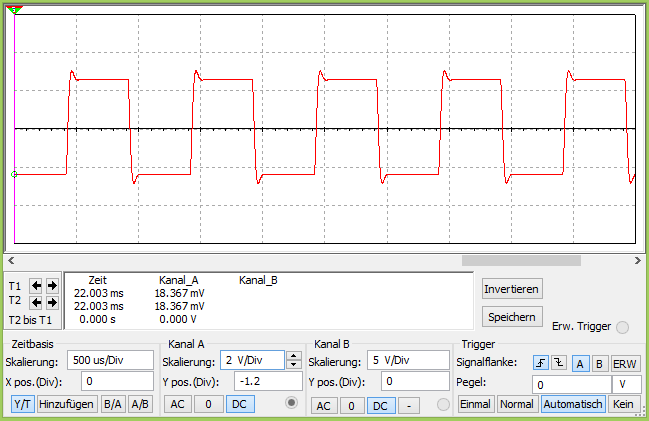
\includegraphics[width=\textwidth , scale = 0.4]{2_3_widerstand_150Ohm.PNG}
                \caption[Aufnahme der Kurve bei 150 $\Omega$]{Aufnahme der Kurve bei 150 $\Omega$}
                \label{fig:23_150}
        \end{subfigure}
       % ~ %add desired spacing between images, e. g. ~, \quad, \qquad, \hfill etc.
          %(or a blank line to force the subfigure onto a new line)
        \hfill
        \begin{subfigure}[b]{0.28\textwidth}
                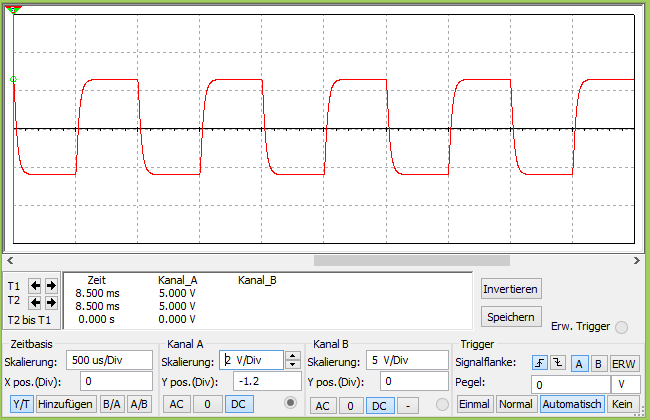
\includegraphics[width=\textwidth , scale = 0.4]{2_3_widerstand_300Ohm.PNG}
                \caption[Aufnahme der Kurve bei 300 $\Omega$]{Aufnahme der Kurve bei 300 $\Omega$}
  				\label{fig:2_3_300}
        \end{subfigure}
        \caption{Kurven  für 50$\Omega$, 150$\Omega$ und 300$\Omega$}
        \label{fig:2_3_1}
\end{figure}


Im zweitem Teil sollte die Auswirkung von R auf die Breite der Resonanzkurve untersucht werden. Dabei ergaben sich die Kurven in Abbildung \ref{fig:2_3_2_1} und Abbildung \ref{fig:2_3_2_2}. Es ist deutlich zu sehen, das bei größerem Widerstand R die Resonanzkurve breiter wird.

\begin{figure}[H]
        \centering
        \begin{subfigure}[b]{0.48\textwidth}
                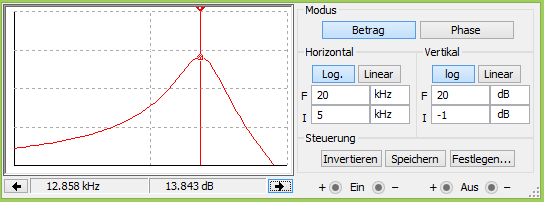
\includegraphics[width=\textwidth , scale = 0.4]{2_3_bode_betrag_25Ohm.PNG}
                \caption[Messung des Frequenzgangs]{Messung des Frequenzgangs}
 				 \label{fig:2_3_25_betrag}
        \end{subfigure}%
        %~ %add desired spacing between images, e. g. ~, \quad, \qquad, \hfill etc.
          %(or a blank line to force the subfigure onto a new line)
        \hfill
        \begin{subfigure}[b]{0.48\textwidth}
                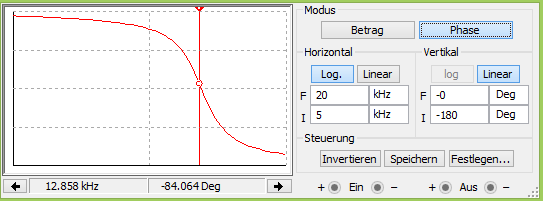
\includegraphics[width=\textwidth , scale = 0.4]{2_3_bode_phase_25Ohm.PNG}
                \caption[Messung des Phasengangs]{Messung des Phasengangs}
  				\label{fig:2_3_25_phase}
        \end{subfigure}
        \caption{Messung des Frequenz- und des Phasengangs bei einem Widerstand von 25$\Omega$}
        \label{fig:2_3_2_1}
\end{figure}


\begin{figure}[H]
        \centering
        \begin{subfigure}[b]{0.48\textwidth}
                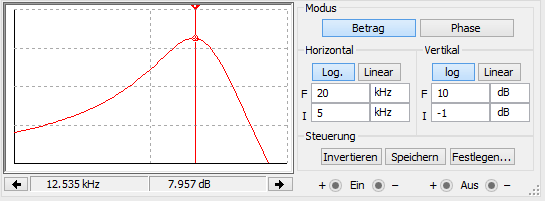
\includegraphics[width=\textwidth , scale = 0.4]{2_3_bode_betrag_50Ohm.PNG}
                \caption[Messung des Frequenzgangs]{Messung des Frequenzgangs}
 				 \label{fig:2_3_25_betrag}
        \end{subfigure}%
        %~ %add desired spacing between images, e. g. ~, \quad, \qquad, \hfill etc.
          %(or a blank line to force the subfigure onto a new line)
        \hfill
        \begin{subfigure}[b]{0.48\textwidth}
                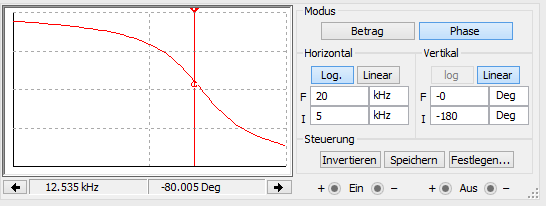
\includegraphics[width=\textwidth , scale = 0.4]{2_3_bode_phase_50Ohm.PNG}
                \caption[Messung des Phasengangs]{Messung des Phasengangs}
  				\label{fig:2_3_25_phase}
        \end{subfigure}
        \caption{Messung des Frequenz- und des Phasengangs bei einem Widerstand von 50$\Omega$}
        \label{fig:2_3_2_2}
\end{figure}

\subsubsection{Diskussion}
%(immer) die gemessenen werte und die bestimmten werte über die messfehler mit literaturwerten oder untereinander vergleichen
%in welchem fehlerintervall des messwertes liegt der literaturwert oder der vergleichswert?
%wie ist der relative anteil des fehlers am messwert und damit die qualität unserer messung?
%in einem satz erklären, wie gut unser fehler und damit unsere messung ist
%kurz erläutern, wie systematische fehler unsere messung beeinflusst haben könnten
%(wichtig) zum schluss ansprechen, in wie weit die ergebnisse mit der theoretischen vorhersage übereinstimmen
%--------------------------------------------------------------------------------------------
%falls tabellen mit den messwerten zu lang werden, kann die section mit den messwerten auch hinter der diskussion angefügt bzw. eine section mit dem anhang eingefügt werden.
%1-----------------------------------------------1

Wie erwartet, wurden bei einem größerem Widerstand R die Überschwinger des Rechtecksignals verkleinert, jedoch kommt es bei einem zu hohem Widerstand zu einer Dämpfung des Signals. Bei der Resonanzfrequenz für ein größerer Widerstand R zu einen breiteren Resonanzkurve, was erwartet wurde.

\section{Simulation mit diskreten aktiven Bauelementen}
In diesem Versuchsteil sollen Simulationen mit Halbleitern durchgeführt werden.

\subsection{Kennlinie einer Siliziumdiode}
%kurz das ziel dieses versuchsteiles ansprechen, damit keine zwei überschriften direkt übereinander stehen!
%bei schwierigeren versuchen kann auch der theoretische hintergrund erläutert werden. (mit formeln, herleitungen und erklärungen)
Die Kennlinie einer Siliziumdiode\footnote{Typ 1N4001GP} wird in diesem Versuchsteil ausgemessen.
\subsubsection{Verwendete Geräte}
%(immer) eine skizze oder ein foto einfügen, die geräte/materialien !nummerieren! und z.b. eine legende dazu schreiben, besser wäre es das ganze in einem Fließtext gut zu beschreiben.
%falls am anfang des versuches nicht klar ist, was alles verwendet wird, wenn möglich erst am ende ein großes foto von den verwendeten materialien machen!\\

Es werden ein Funktionsgenerator, ein Widerstand, eine Siliziumdiode und ein Oszilloskop verwendet.(Multisim)


\subsubsection{Versuchsaufbau}
%skizze zum versuchsaufbau (oder foto) einfügen,   es muss erklärt werden wie das ganze funktioniert und welche speziellen einstellungen verwendet wurden (z.b. welche knöpfe an den geräten für die messung verdreht wurden)

R1 ist ein 1k$\Omega$ Widerstand und die Siliziumdiode ist eine 1N4001 Diode.


\begin{figure}[H] 
  \centering
    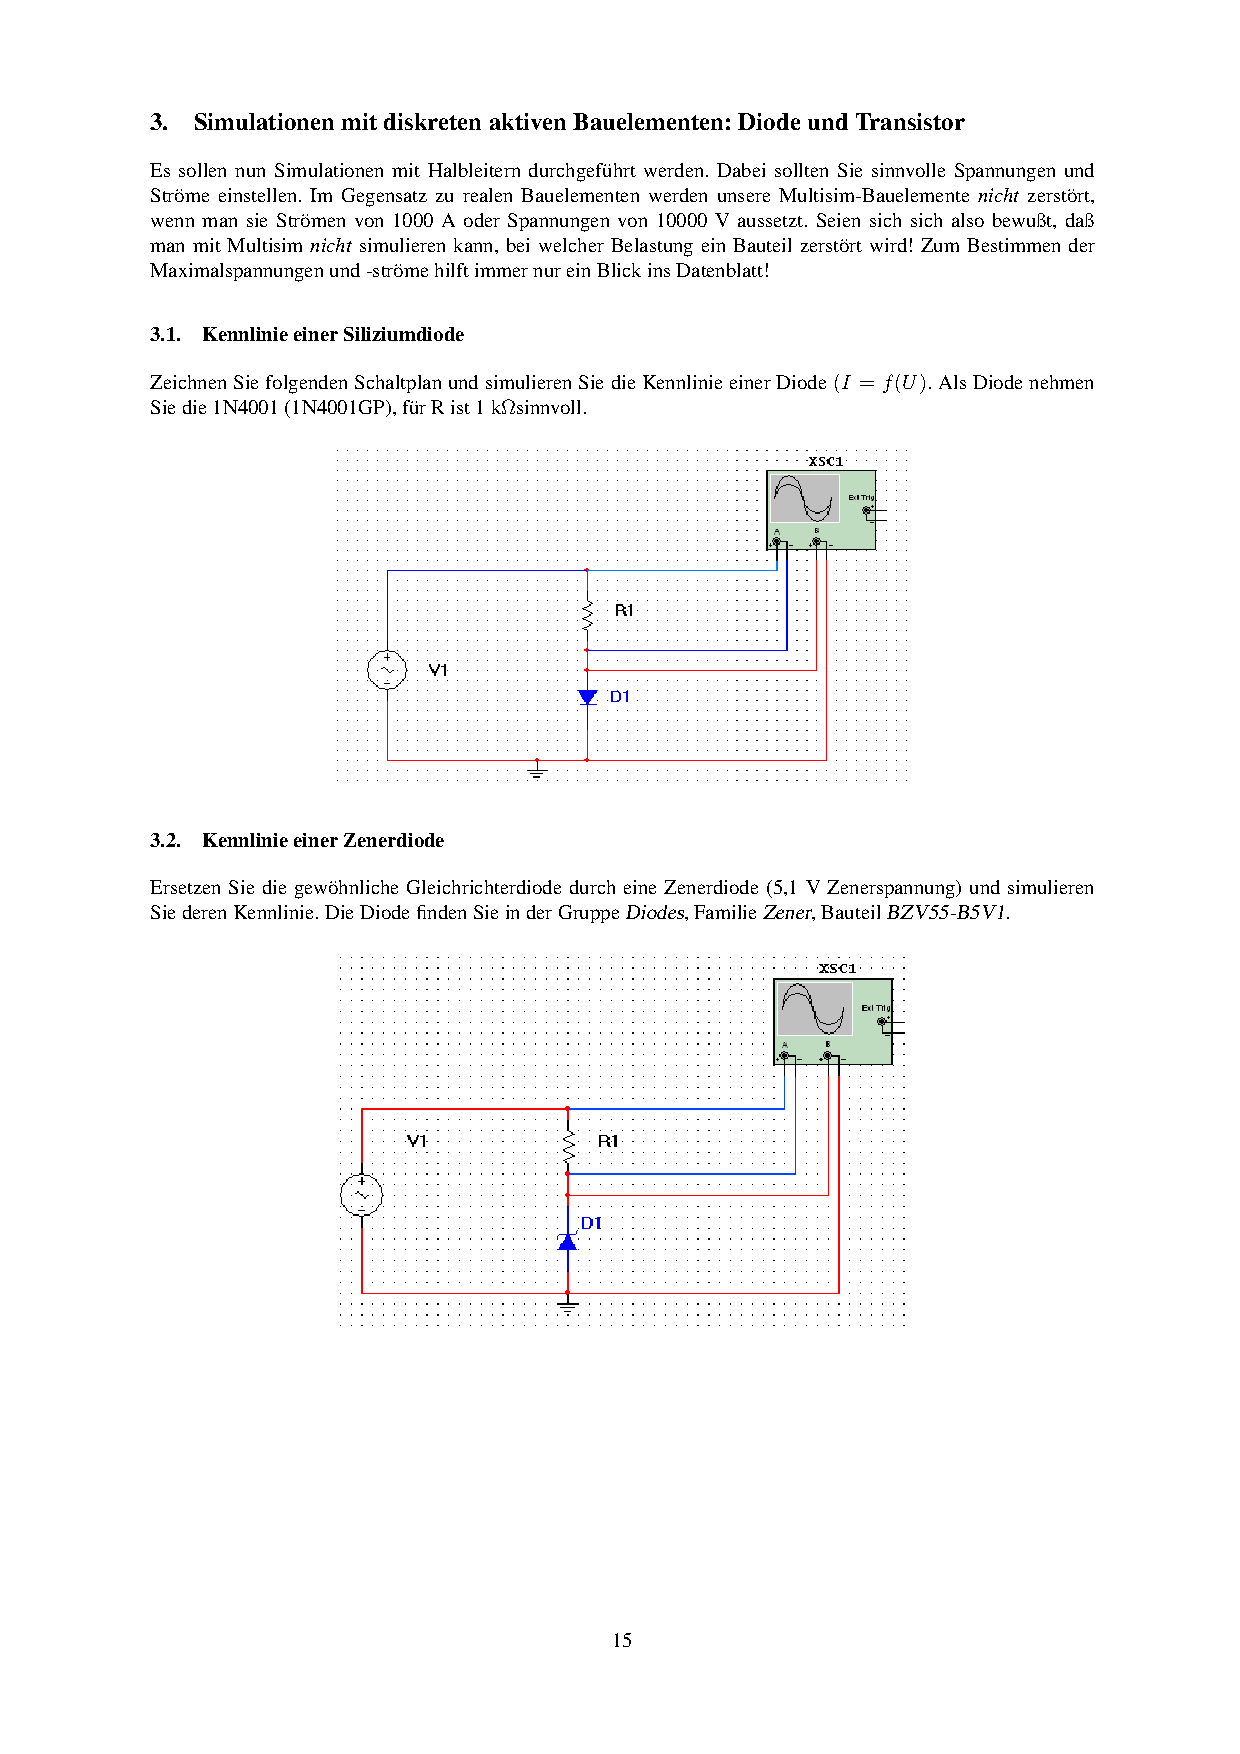
\includegraphics[trim = 10mm 160mm 10mm 75mm, clip, scale = 1]{ep5_14[Page15].pdf}
  	\caption[Schaltskizze zur Aufnahme der Diodenkennlinie (Siliziumdiode)]{Schaltskizze zur Aufnahme der Diodenkennlinie (Siliziumdiode)\footnotemark}
  \label{fig:3.1}
\end{figure}
\footnotetext{Abbildung entnommen von http://www.atlas.uni-wuppertal.de/$\sim$kind/ep5\_14.pdf Seite 15 am 22.11.2014}

\subsubsection{Versuchsdurchführung}
%erklären, !was! wir machen, !warum! wir das machen und mit welchem ziel
%(wichtig) präzize erklären, wie bei dem versuch vorgegangen und was gemacht wurde
Die Schaltung wird nach dem Schaltplan Abbildung \ref{fig:3.1} in Multisim zusammengebaut. Am Oszilloskop kann die Kennlinie abgelesen werden.
\subsubsection{Auswertung}
%zuerst !alle! errechneten werte entweder in ganzen sätzen aufzählen, oder in tabellen (übersichtlicher) dargestellen, sowie auf die verwendeten formeln verweisen (die referenzierung der formel kann in der überschrift stehen)
%kurz erwähnen (vor der tabelle), warum wir das ganze ausrechnen bzw. was wir dort ausrechnen
%danach histogramme und plots erstellen, wobei wenn möglich funktionen durch die plots gelegt werden (zur not können auch splines benutzt werden, was aber angegeben werden muss)
%bei fits immer die funktion und das reduzierte chiquadrat mit angegeben, wobei auf verständlichkeit beim entziffern der zehnerpotenzen geachtet werden muss z.b. f(x)=(wert+-fehler)\cdot10^{irgendeine zahl}\cdot x + (wert+-fehler)\cdot10^{irgendeine zahl}
%bei jedem fit erklären, nach welchem zusammenhang gefittet wurde und warum!
%bei plots darauf achten, dass die achsenbeschriftung (auch die tics) die richtige größe haben und die legende im plot nicht die messwerte verdeckt
%kurz die aufgabenstellung abhandeln
%2-----------------------------------------------2
Mit dem Oszilloskop wurde die Diodenkennlinie mit einem Sinussignal durchgefahren.
Wie man sieht hat die Diode auch geringe Kapazitive Eigenschaften.
\begin{figure}[H] 
  \centering
    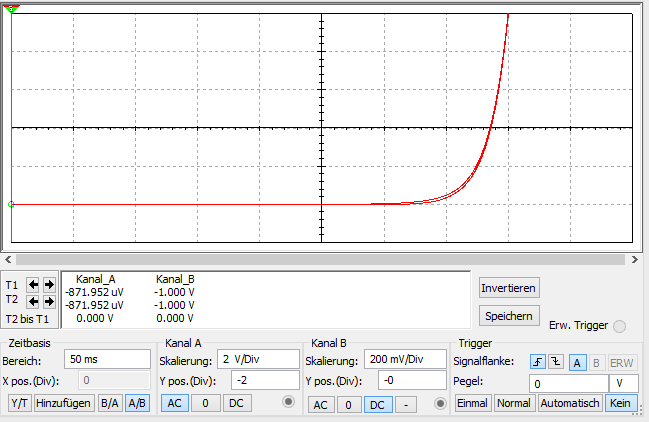
\includegraphics[trim = 0mm 0mm 0mm 0mm, clip, scale = 1]{3_1_kennlinie.PNG}
  	\caption[Diodenkennlinie am Oszilloskop (Siliziumdiode)]{Diodenkennlinie am Oszilloskop (Siliziumdiode)}
  \label{fig:Diodenkennlinie_Oszilloskop_Siliziumdiode}
\end{figure}
\subsubsection{Diskussion}
%(immer) die gemessenen werte und die bestimmten werte über die messfehler mit literaturwerten oder untereinander vergleichen
%in welchem fehlerintervall des messwertes liegt der literaturwert oder der vergleichswert?
%wie ist der relative anteil des fehlers am messwert und damit die qualität unserer messung?
%in einem satz erklären, wie gut unser fehler und damit unsere messung ist
%kurz erläutern, wie systematische fehler unsere messung beeinflusst haben könnten
%(wichtig) zum schluss ansprechen, in wie weit die ergebnisse mit der theoretischen vorhersage übereinstimmen
%--------------------------------------------------------------------------------------------
%falls tabellen mit den messwerten zu lang werden, kann die section mit den messwerten auch hinter der diskussion angefügt bzw. eine section mit dem anhang eingefügt werden.
%1-----------------------------------------------1
Der erwartete exponentielle Zusammenhang kann an Abbildung \ref{fig:Diodenkennlinie_Oszilloskop_Siliziumdiode} abgelesen werden.
Die Diode hat bei Wechselspannung auch Kapazitive Eigenschaften, sodass eine leichte Verschiebung der Kennlinie entsteht.



\subsection{Kennlinie einer Zenerdiode}
%kurz das ziel dieses versuchsteiles ansprechen, damit keine zwei überschriften direkt übereinander stehen!
%bei schwierigeren versuchen kann auch der theoretische hintergrund erläutert werden. (mit formeln, herleitungen und erklärungen)
In diesem Versuchsteil wird die Kennlinie einer Zenerdiode mit dem Oszilloskop aufgenommen.
\subsubsection{Verwendete Geräte}
%(immer) eine skizze oder ein foto einfügen, die geräte/materialien !nummerieren! und z.b. eine legende dazu schreiben, besser wäre es das ganze in einem Fließtext gut zu beschreiben.
%falls am anfang des versuches nicht klar ist, was alles verwendet wird, wenn möglich erst am ende ein großes foto von den verwendeten materialien machen!\\

Es werden ein Funktionsgenerator, ein Widerstand, eine Zenerdiode und ein Oszilloskop verwendet.(Multisim)

\subsubsection{Versuchsaufbau}
%skizze zum versuchsaufbau (oder foto) einfügen,   es muss erklärt werden wie das ganze funktioniert und welche speziellen einstellungen verwendet wurden (z.b. welche knöpfe an den geräten für die messung verdreht wurden)

R1 ist ein 1k$\Omega$ Widerstand und die Zenerdiode ist eine BZV55-B5V1 Diode.


\begin{figure}[H] 
  \centering
    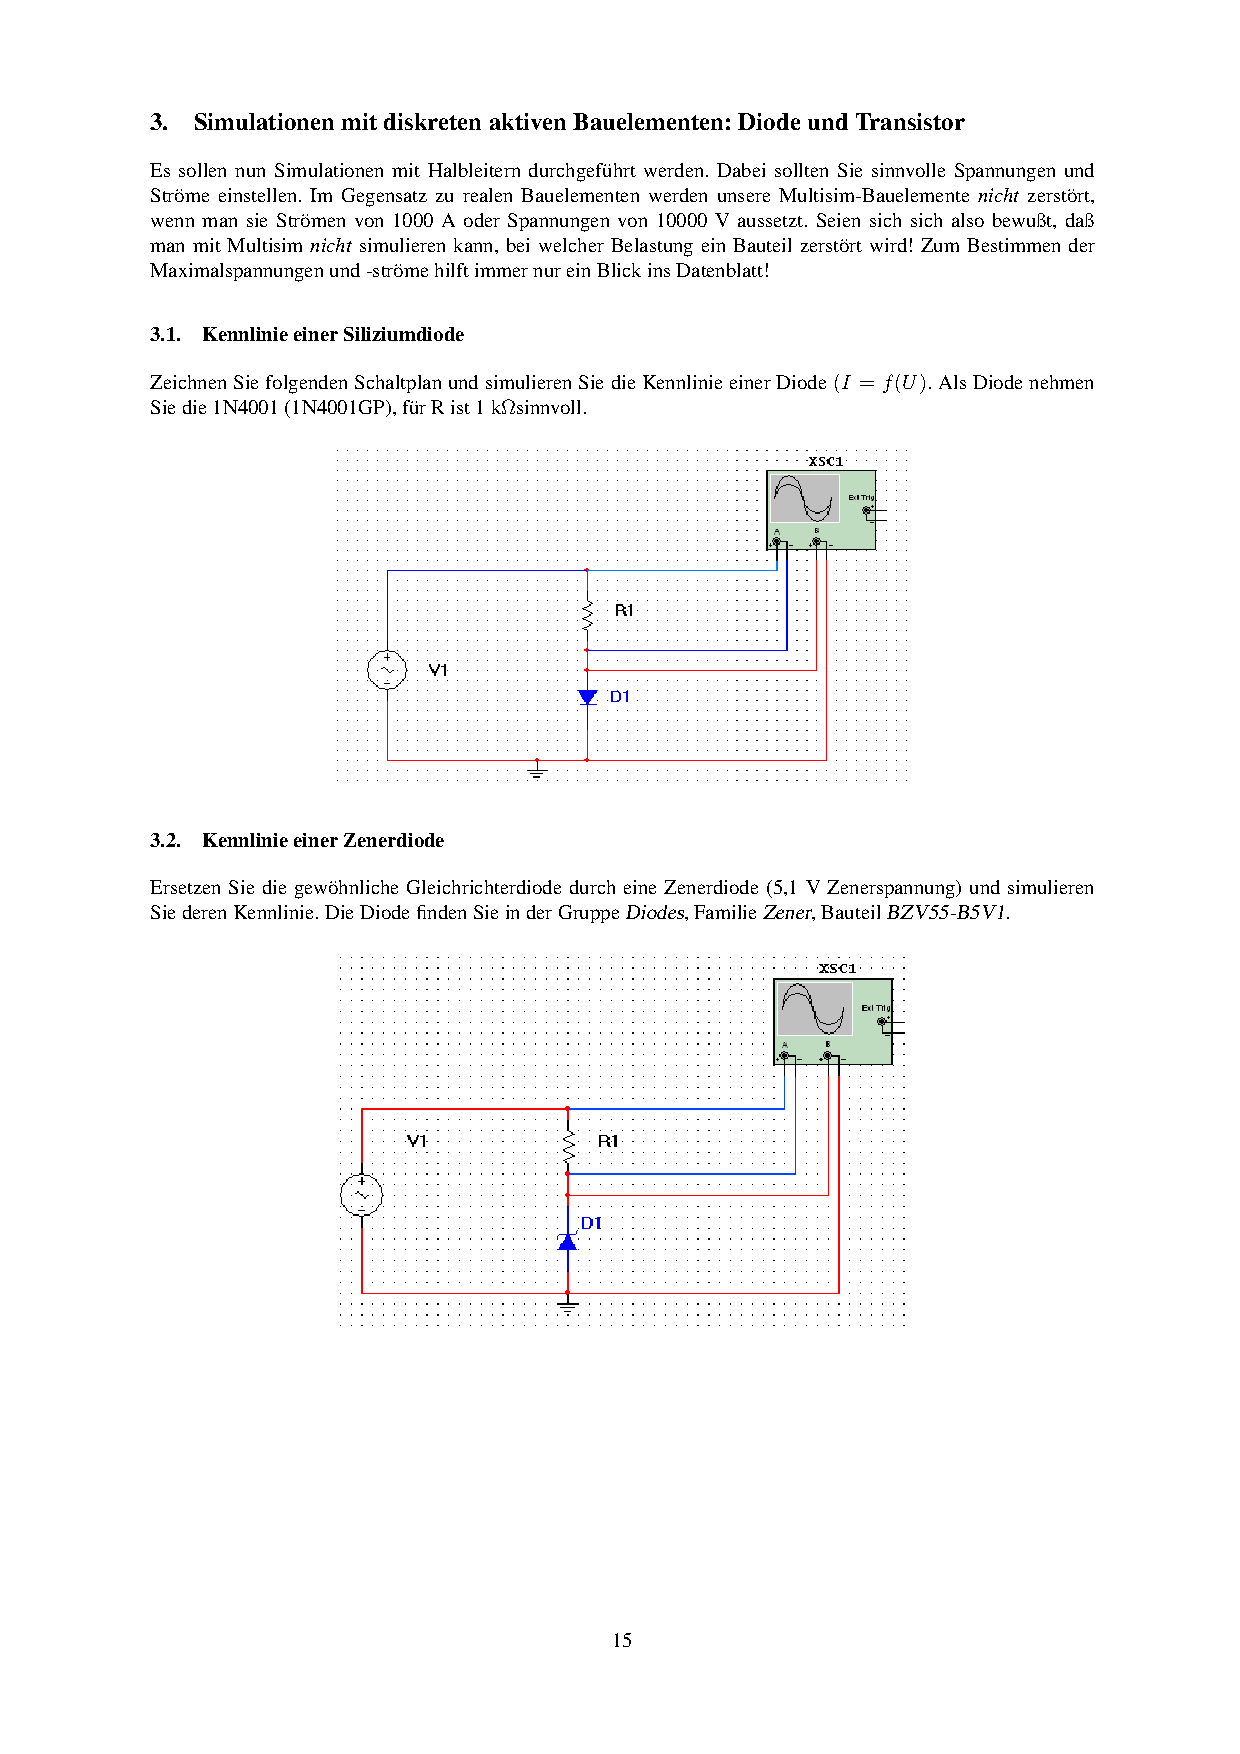
\includegraphics[trim = 10mm 70mm 10mm 165mm, clip, scale = 1]{ep5_14[Page15].pdf}
  	\caption[Schaltskizze zur Aufnahme der Diodenkennlinie (Zenerdiode)]{Schaltskizze zur Aufnahme der Diodenkennlinie (Zenerdiode)\footnotemark}
  \label{fig:3.2}
\end{figure}
\footnotetext{Abbildung entnommen von http://www.atlas.uni-wuppertal.de/$\sim$kind/ep5\_14.pdf Seite 15 am 22.11.2014}

\subsubsection{Versuchsdurchführung}
%erklären, !was! wir machen, !warum! wir das machen und mit welchem ziel
%(wichtig) präzize erklären, wie bei dem versuch vorgegangen und was gemacht wurde
Die Zenerdiode Typ BZV55-B5V1 hat entsprechend eine Zenerspannung von \unit[5,1]{V}.
Die Kennlinie wird nach Schaltung Abb. \ref{fig:3.2} mit dem Oszilloskop aufgenommen. In Multisim wird der Schaltplan gemäß Abb. \ref{fig:3.2} eingezeichnet.
\subsubsection{Auswertung}
%zuerst !alle! errechneten werte entweder in ganzen sätzen aufzählen, oder in tabellen (übersichtlicher) dargestellen, sowie auf die verwendeten formeln verweisen (die referenzierung der formel kann in der überschrift stehen)
%kurz erwähnen (vor der tabelle), warum wir das ganze ausrechnen bzw. was wir dort ausrechnen
%danach histogramme und plots erstellen, wobei wenn möglich funktionen durch die plots gelegt werden (zur not können auch splines benutzt werden, was aber angegeben werden muss)
%bei fits immer die funktion und das reduzierte chiquadrat mit angegeben, wobei auf verständlichkeit beim entziffern der zehnerpotenzen geachtet werden muss z.b. f(x)=(wert+-fehler)\cdot10^{irgendeine zahl}\cdot x + (wert+-fehler)\cdot10^{irgendeine zahl}
%bei jedem fit erklären, nach welchem zusammenhang gefittet wurde und warum!
%bei plots darauf achten, dass die achsenbeschriftung (auch die tics) die richtige größe haben und die legende im plot nicht die messwerte verdeckt
%kurz die aufgabenstellung abhandeln
%2-----------------------------------------------2
Die Zenerdiodenkennline wurde mit dem Oszilloskop aufgenommen wie man in Abbildung \ref{fig:3.2_Aufnahme_Diodenkennlinie} sieht. Als Spitzenspannung wurde \unit[30]{V} verwendet.
\begin{figure}[H] 
  \centering
    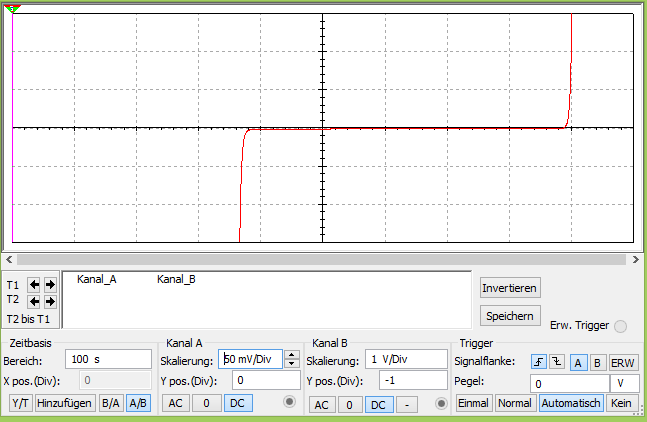
\includegraphics[trim = 0mm 0mm 0mm 0mm, clip, scale = 1]{3_2_kennlinie.PNG}
  	\caption[Aufnahme der Diodenkennlinie (Zenerdiode)]{Aufnahme der Diodenkennlinie (Zenerdiode)}
  \label{fig:3.2_Aufnahme_Diodenkennlinie}
\end{figure}
Es ist zu beobachten, dass die Spannung über dem Widerstand bei der Durchbruchspannung \unit[5,1]{V} sehr steil abknickt.
\subsubsection{Diskussion}
%(immer) die gemessenen werte und die bestimmten werte über die messfehler mit literaturwerten oder untereinander vergleichen
%in welchem fehlerintervall des messwertes liegt der literaturwert oder der vergleichswert?
%wie ist der relative anteil des fehlers am messwert und damit die qualität unserer messung?
%in einem satz erklären, wie gut unser fehler und damit unsere messung ist
%kurz erläutern, wie systematische fehler unsere messung beeinflusst haben könnten
%(wichtig) zum schluss ansprechen, in wie weit die ergebnisse mit der theoretischen vorhersage übereinstimmen
%--------------------------------------------------------------------------------------------
%falls tabellen mit den messwerten zu lang werden, kann die section mit den messwerten auch hinter der diskussion angefügt bzw. eine section mit dem anhang eingefügt werden.
%1-----------------------------------------------1
Es wurde die erwartete Durchbruchspannung bei \unit[5,1]{V} mit dem Oszilloskop aufgenommen. 

\subsection{Kennlinie eines Transistors}
%kurz das ziel dieses versuchsteiles ansprechen, damit keine zwei überschriften direkt übereinander stehen!
%bei schwierigeren versuchen kann auch der theoretische hintergrund erläutert werden. (mit formeln, herleitungen und erklärungen)
In diesem Versuchsteil wird die Eingangs- und Ausgangskennlinie des Transistors aufgenommen.
\subsubsection{Verwendete Geräte}
%(immer) eine skizze oder ein foto einfügen, die geräte/materialien !nummerieren! und z.b. eine legende dazu schreiben, besser wäre es das ganze in einem Fließtext gut zu beschreiben.
%falls am anfang des versuches nicht klar ist, was alles verwendet wird, wenn möglich erst am ende ein großes foto von den verwendeten materialien machen!\\

Es werden ein Funktionsgenerator, ein Widerstand, ein Transistor und ein Oszilloskop verwendet.(Multisim)

\subsubsection{Versuchsaufbau}
%skizze zum versuchsaufbau (oder foto) einfügen,   es muss erklärt werden wie das ganze funktioniert und welche speziellen einstellungen verwendet wurden (z.b. welche knöpfe an den geräten für die messung verdreht wurden)

Im ersten Aufbau ist R1 ist ein 1k$\Omega$ Widerstand und der Transistor ist ein BC550 Transistor. Im zweitem Aufbau ist R1 ein 100k$\Omega$ und R2 ein 100$\Omega$ Widerstand.


\begin{figure}[H]
        \centering
        \begin{subfigure}[t]{0.48\textwidth}
               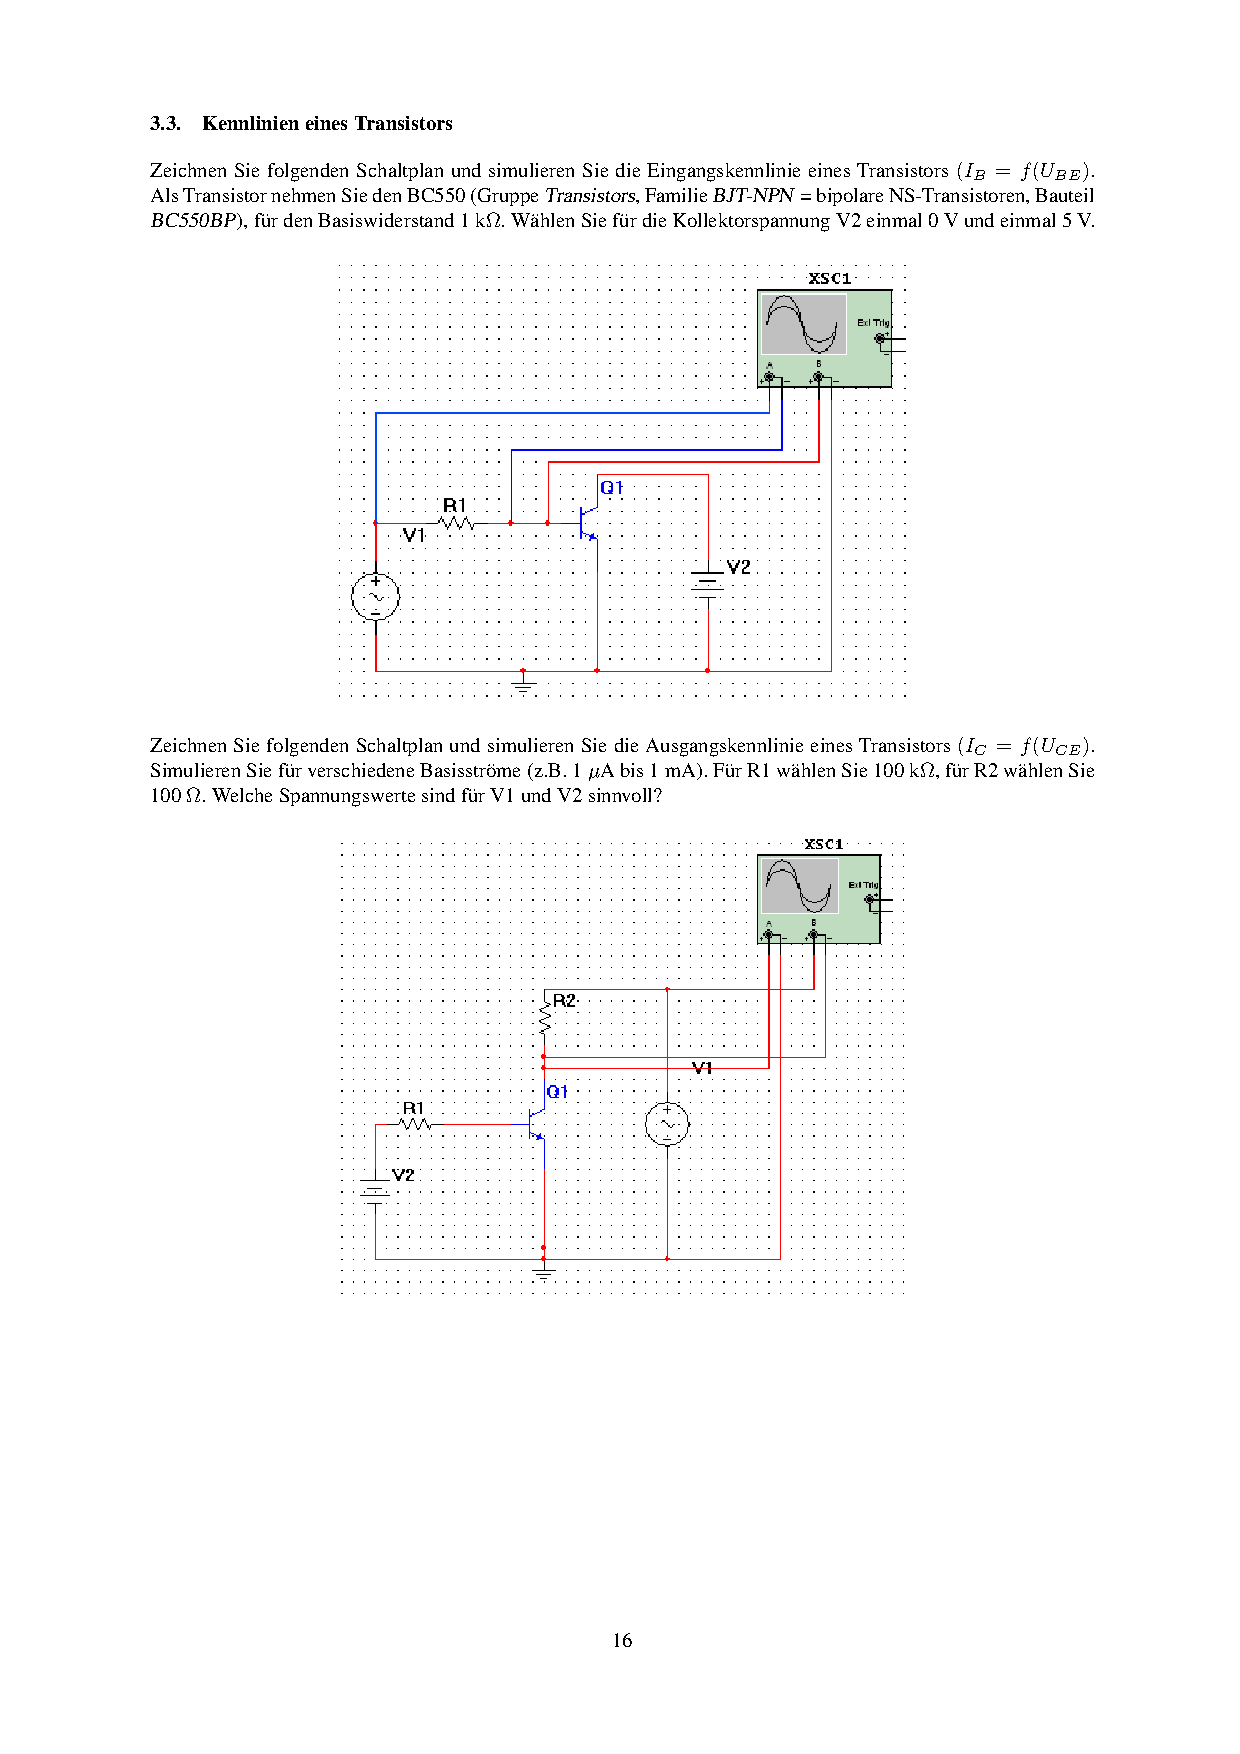
\includegraphics[trim = 30mm 175mm 30mm 40mm, clip, scale = 0.7]{ep5_14[Page16].pdf}
				\caption[Schaltskizze zur Aufnahme der Eingangskennlinie eines BC550 Transistors]{Schaltskizze zur Aufnahme der Kennlinie eines BC550 Transistors\footnotemark}
 				 \label{fig:3.31}
        \end{subfigure}%
        %~ %add desired spacing between images, e. g. ~, \quad, \qquad, \hfill etc.
          %(or a blank line to force the subfigure onto a new line)
        \hfill
        \begin{subfigure}[t]{0.48\textwidth}
                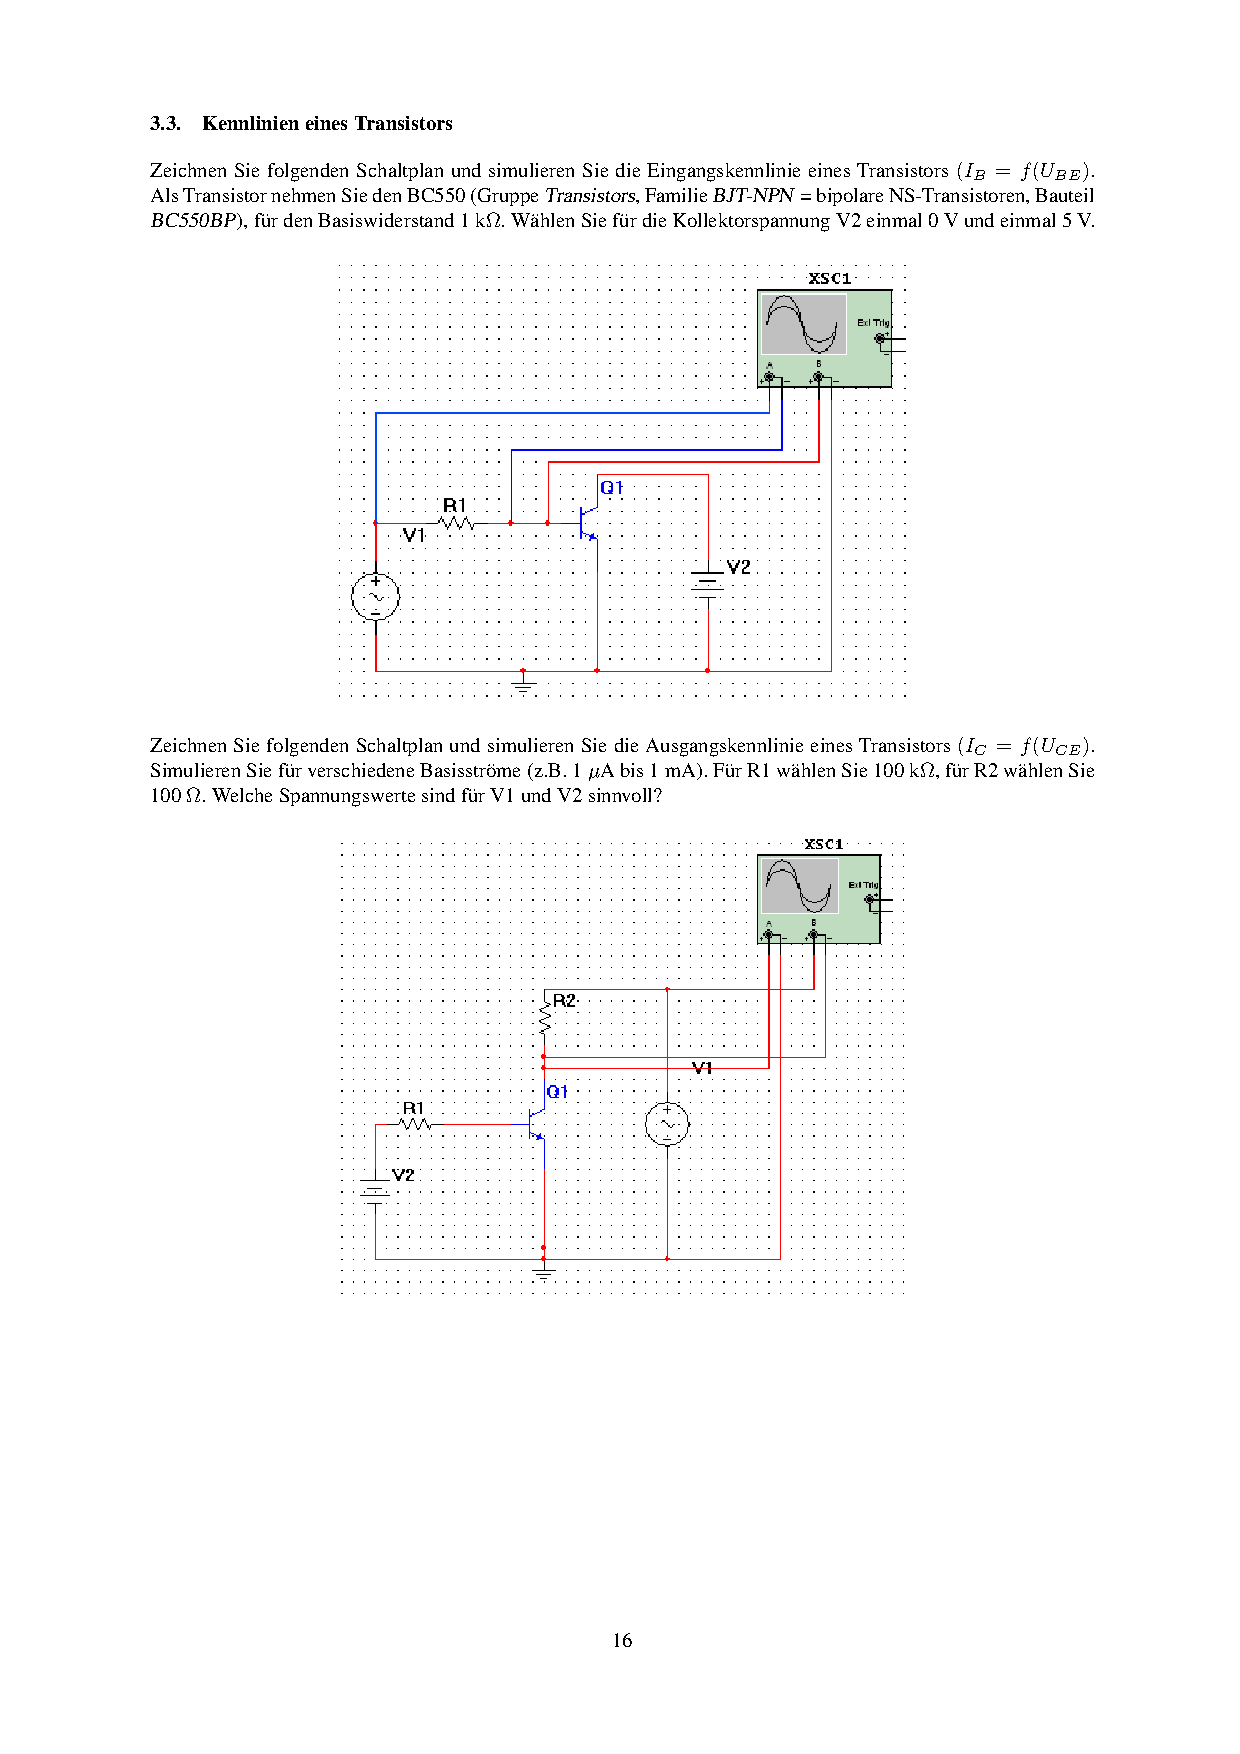
\includegraphics[trim = 30mm 75mm 30mm 140mm, clip, scale = 0.7]{ep5_14[Page16].pdf}
  				\caption[Schaltskizze zur Aufnahme der Augangskennlinie eines BC550 Transistors]{Schaltskizze zur Aufnahme der Kennlinie eines BC550 Transistors\footnotemark}
  				\label{fig:3.32}
        \end{subfigure}
        \caption{Aufbauten zur Messung der Transistorkennlinie}
        \label{fig:3.3}
\end{figure}


\subsubsection{Versuchsdurchführung}
%erklären, !was! wir machen, !warum! wir das machen und mit welchem ziel
%(wichtig) präzize erklären, wie bei dem versuch vorgegangen und was gemacht wurde
Zuerst wird der Schaltplan für die Eingangskennlinie gemäß Abb. \ref{fig:3.31} in Multisim eingezeichnet, welche dann mit dem Oszilloskop aufgenommen werden soll. Es wird ein Transistor vom Typ  BC550 und ein Basiswiderstand von \unit[1]{k$\Omega$} verwendet. Als zweites wird der Schaltplan gemäß Abb. \ref{fig:3.32} in Multisim eingezeichnet und simuliert.(R1 = \unit[100]{k$\Omega$}, R2 = \unit[100]{$\Omega$})
Die Ausgangskennlinie wird mit dem Oszilloskop aufgenommen.
\subsubsection{Auswertung}
%zuerst !alle! errechneten werte entweder in ganzen sätzen aufzählen, oder in tabellen (übersichtlicher) dargestellen, sowie auf die verwendeten formeln verweisen (die referenzierung der formel kann in der überschrift stehen)
%kurz erwähnen (vor der tabelle), warum wir das ganze ausrechnen bzw. was wir dort ausrechnen
%danach histogramme und plots erstellen, wobei wenn möglich funktionen durch die plots gelegt werden (zur not können auch splines benutzt werden, was aber angegeben werden muss)
%bei fits immer die funktion und das reduzierte chiquadrat mit angegeben, wobei auf verständlichkeit beim entziffern der zehnerpotenzen geachtet werden muss z.b. f(x)=(wert+-fehler)\cdot10^{irgendeine zahl}\cdot x + (wert+-fehler)\cdot10^{irgendeine zahl}
%bei jedem fit erklären, nach welchem zusammenhang gefittet wurde und warum!
%bei plots darauf achten, dass die achsenbeschriftung (auch die tics) die richtige größe haben und die legende im plot nicht die messwerte verdeckt
%kurz die aufgabenstellung abhandeln
%2-----------------------------------------------2
Die Eingangskennlinie des Transistors wurde mit dem Oszilloskop aufgenommen.
\begin{figure}[H]
        \centering
        \begin{subfigure}[t]{0.48\textwidth}
               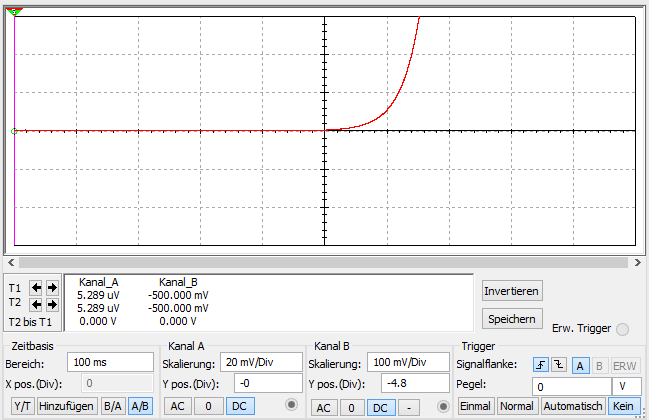
\includegraphics[trim = 0mm 0mm 0mm 0mm, clip, scale = 0.5]{3_3_eingangskennlinie_0Volt.PNG}
				\caption[Aufnahme der Eingangskennlinie eines BC550 Transistors bei einer Kollektorspannung von 0 V]{Aufnahme der Eingangskennlinie eines BC550 Transistors bei einer Kollektorspannung von 0 V}
 				 \label{fig:3.311}
        \end{subfigure}%
        %~ %add desired spacing between images, e. g. ~, \quad, \qquad, \hfill etc.
          %(or a blank line to force the subfigure onto a new line)
        \hfill
        \begin{subfigure}[t]{0.48\textwidth}
                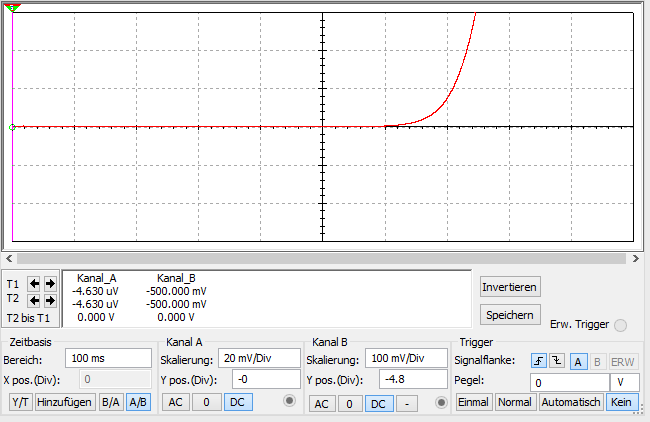
\includegraphics[trim = 0mm 0mm 0mm 0mm, clip, scale = 0.5]{3_3_eingangskennlinie_5Volt.PNG}
  				\caption[Aufnahme der Eingangskennlinie eines BC550 Transistors bei einer Kollektorspannung von 5 V]{Aufnahme der Eingangskennlinie eines BC550 Transistors bei einer Kollektorspannung von 5V}
  				\label{fig:3.312}
        \end{subfigure}
        \caption{Aufbauten zur Messung der Transistorkennlinie}
        \label{fig:3.31_Auswertung}
\end{figure}
Beobachtet wurde das typische Verhalten einer Diode, wie man an Abb. \ref{fig:3.311} und \ref{fig:3.312} sieht. Die Kennlinien wurden um \unit[480]{mV} nach links verschoben.\newline
Bei der Aufnahme der Ausgangskennlinie wurde eine Spitzenspannung von \unit[1]{V} und für V2 wurde 0,7 und \unit[0,8]{V} verwendet. 
\begin{figure}[H]
        \centering
        \begin{subfigure}[t]{0.48\textwidth}
               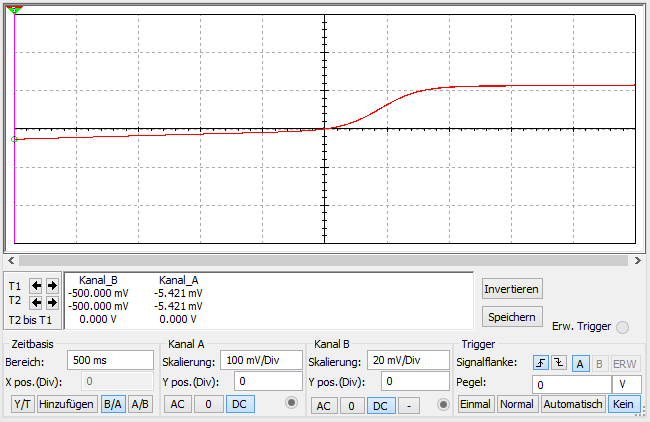
\includegraphics[trim = 0mm 0mm 0mm 0mm, clip, scale = 0.5]{3_3_ausgangskennlinie_0,7V.PNG}
				\caption[Aufnahme der Ausgangskennlinie eines BC550 Transistors bei einer Spannung V1 von 0,7 V]{Aufnahme der Ausgangskennlinie eines BC550 Transistors bei einer Spannung V1 von 0,7 V}
 				 \label{fig:3.321}
        \end{subfigure}%
        %~ %add desired spacing between images, e. g. ~, \quad, \qquad, \hfill etc.
          %(or a blank line to force the subfigure onto a new line)
        \hfill
        \begin{subfigure}[t]{0.48\textwidth}
                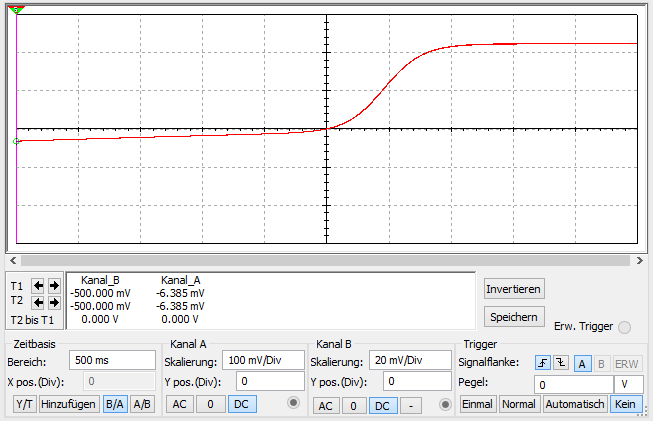
\includegraphics[trim = 0mm 0mm 0mm 0mm, clip, scale = 0.5]{3_3_ausgangskennlinie_0,8V.PNG}
  				\caption[Aufnahme der Ausgangskennlinie eines BC550 Transistors bei einer Spannung V1 von 0,8 V]{Aufnahme der Ausgangskennlinie eines BC550 Transistors bei einer Spannung V1 von 0,8 V}
  				\label{fig:3.322}
        \end{subfigure}
        \caption{Aufbauten zur Messung der Transistorkennlinie}
        \label{fig:3.32_Auswertung}
\end{figure}
\subsubsection{Diskussion}
%(immer) die gemessenen werte und die bestimmten werte über die messfehler mit literaturwerten oder untereinander vergleichen
%in welchem fehlerintervall des messwertes liegt der literaturwert oder der vergleichswert?
%wie ist der relative anteil des fehlers am messwert und damit die qualität unserer messung?
%in einem satz erklären, wie gut unser fehler und damit unsere messung ist
%kurz erläutern, wie systematische fehler unsere messung beeinflusst haben könnten
%(wichtig) zum schluss ansprechen, in wie weit die ergebnisse mit der theoretischen vorhersage übereinstimmen
%--------------------------------------------------------------------------------------------
%falls tabellen mit den messwerten zu lang werden, kann die section mit den messwerten auch hinter der diskussion angefügt bzw. eine section mit dem anhang eingefügt werden.
%1-----------------------------------------------1
Die Basis-Emitter-Diodenkennlinie wurde mit dem Oszilloskop bei verschiedenen Kollektorspannungen aufgenommen. Wie erwartet verschiebt sich die Kennlinie bei größerer Kollektorspannung nach rechts, da ein Teil der Elektronen von der Kollektorspannung abgesaugt wird. Die Kennlinien in Abb. \ref{fig:3.31_Auswertung} wurden um \unit[480]{mV} nach links verschoben. Die Ausgangskennlinie wurde mit mit den Spannungen V2 von 0,7 und \unit[0,8]{V} aufgenommen und ergeben die erwarteten Kurven, wie man in Abb. \ref{fig:3.32_Auswertung} sieht. 

\subsection{Transistorverstärker}
%kurz das ziel dieses versuchsteiles ansprechen, damit keine zwei überschriften direkt übereinander stehen!
%bei schwierigeren versuchen kann auch der theoretische hintergrund erläutert werden. (mit formeln, herleitungen und erklärungen)
\subsubsection{Verwendete Geräte}
%(immer) eine skizze oder ein foto einfügen, die geräte/materialien !nummerieren! und z.b. eine legende dazu schreiben, besser wäre es das ganze in einem Fließtext gut zu beschreiben.
%falls am anfang des versuches nicht klar ist, was alles verwendet wird, wenn möglich erst am ende ein großes foto von den verwendeten materialien machen!\\

Es werden ein Funktionsgenerator, Widerstände, Kondensatoren, ein Transistor und ein Oszilloskop verwendet.

\subsubsection{Verwendete Formeln}
%eine legende kann angefertigt werden, die selbstverständlichen buchstaben müssen nicht extra erklärt werden
%mit knappen erklärungen die !verwendeten! formeln, sowie die zugehörige fehlerrechnung einfügen
%2-----------------------------------------------2
%ab hier kann nochmal in einzelne versuchsteile unterteilt werden
\subsubsection{Versuchsaufbau}
%skizze zum versuchsaufbau (oder foto) einfügen,   es muss erklärt werden wie das ganze funktioniert und welche speziellen einstellungen verwendet wurden (z.b. welche knöpfe an den geräten für die messung verdreht wurden)

R1 ist ein 1k$\Omega$ Widerstand, R2 ist ein 1M$\Omega$ Widerstand und R3 ist ein 10k$\Omega$ Widerstand. C1 ist ein 100nF Kondensator und C2 ein 1$\mu$F Kondensator.


\begin{figure}[H] 
  \centering
    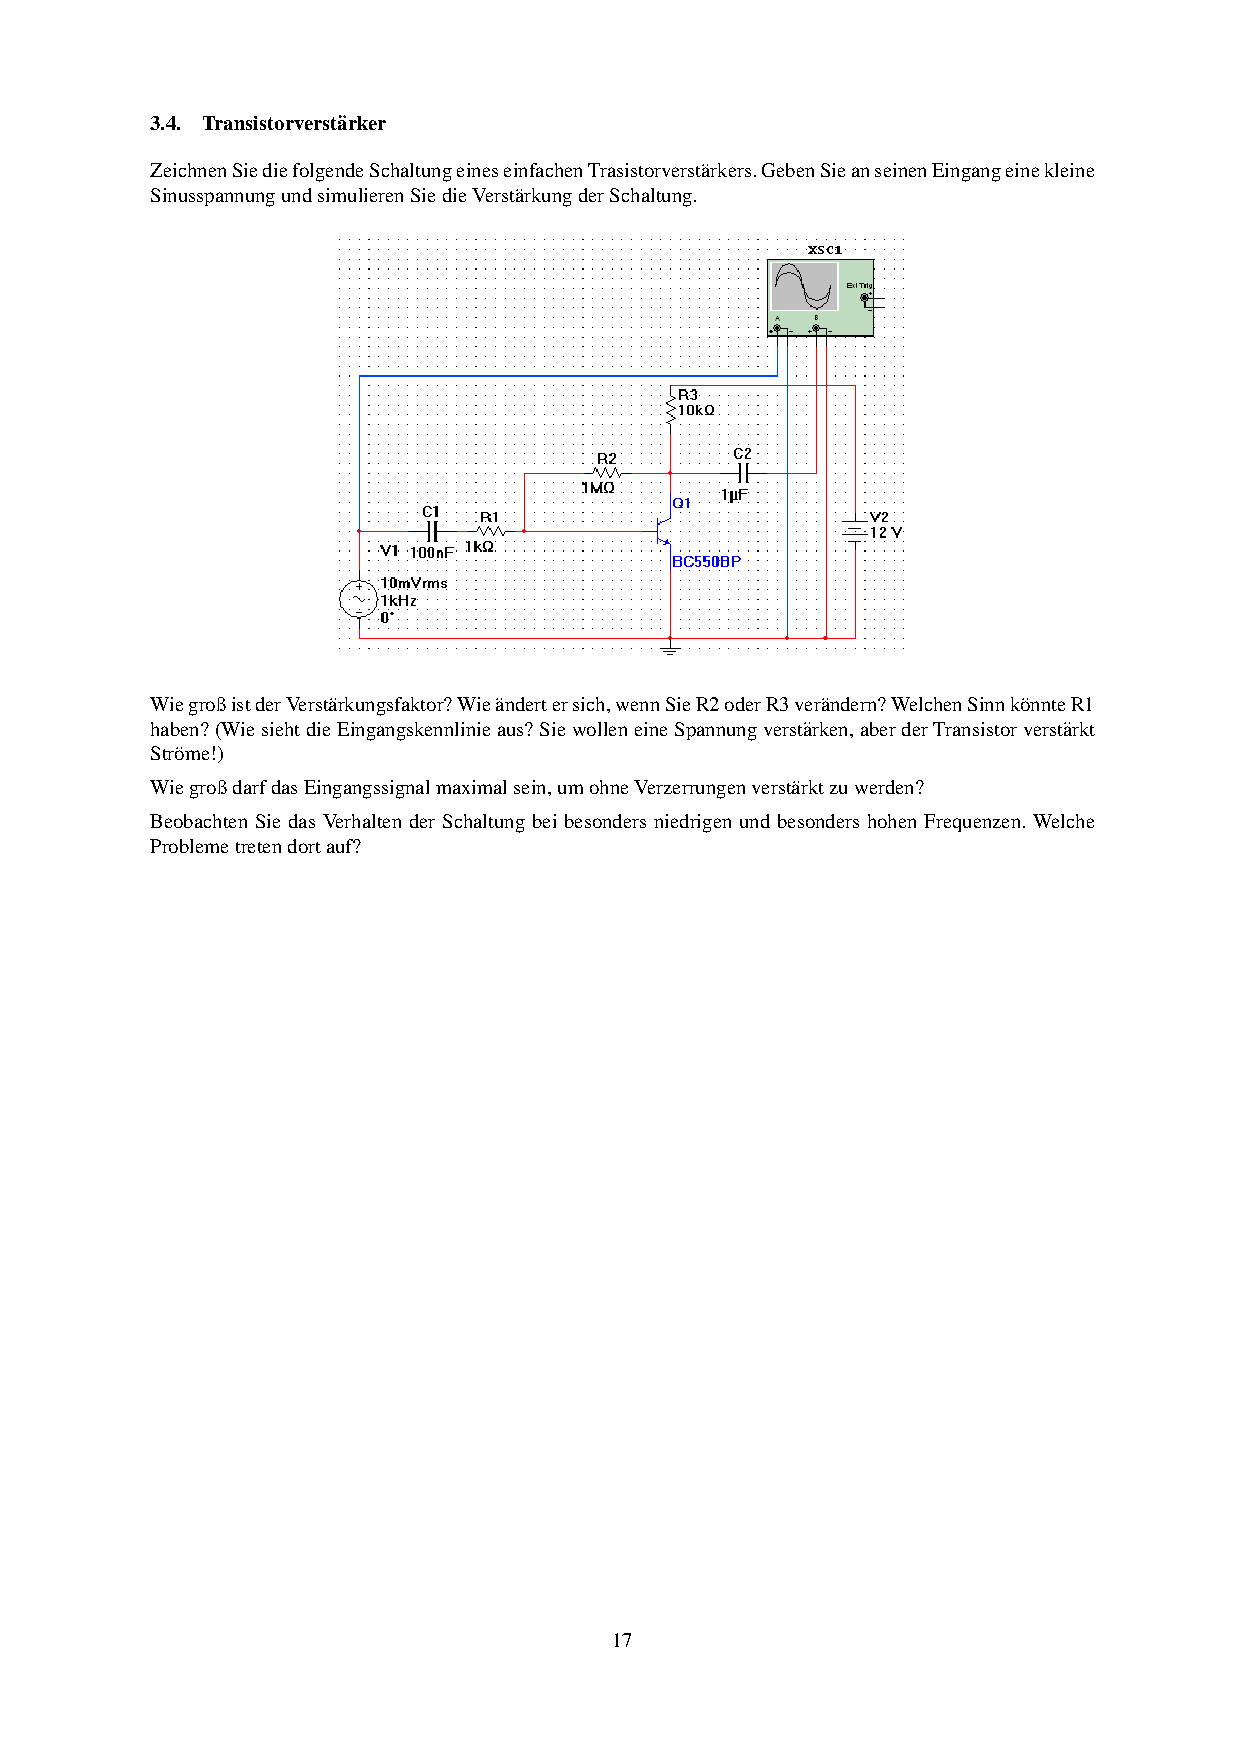
\includegraphics[trim = 10mm 180mm 10mm 40mm, clip, scale = 1]{ep5_14[Page17].pdf}
  	\caption[Schaltskizze für eine Transistorverstärkung]{Schaltskizze für eine Transistorverstärkung\footnotemark}
  \label{fig:1}
\end{figure}
\footnotetext{Abbildung entnommen von http://www.atlas.uni-wuppertal.de/$\sim$kind/ep5\_14.pdf Seite 17 am 22.11.2014}

\subsubsection{Versuchsdurchführung}
%erklären, !was! wir machen, !warum! wir das machen und mit welchem ziel
%(wichtig) präzize erklären, wie bei dem versuch vorgegangen und was gemacht wurde

\subsubsection{Messergebnisse}
%die messwerte in !übersichtlichen! tabellen angegeben
%zu viele kleine tabellen in große tabellen überführen!
%zu große tabellen mit dem [scale]-befehl scalieren oder (falls zu lang) in zwei kleinere tabellen aufteilen
%(wichtig) vor !jeder! tabelle sagen, was gemessen wurde und wie die fehler gewählt wurden und ausreichend !erklären!, !warum! wir unsere fehler grade so gewählt haben
\subsubsection{Auswertung}
%zuerst !alle! errechneten werte entweder in ganzen sätzen aufzählen, oder in tabellen (übersichtlicher) dargestellen, sowie auf die verwendeten formeln verweisen (die referenzierung der formel kann in der überschrift stehen)
%kurz erwähnen (vor der tabelle), warum wir das ganze ausrechnen bzw. was wir dort ausrechnen
%danach histogramme und plots erstellen, wobei wenn möglich funktionen durch die plots gelegt werden (zur not können auch splines benutzt werden, was aber angegeben werden muss)
%bei fits immer die funktion und das reduzierte chiquadrat mit angegeben, wobei auf verständlichkeit beim entziffern der zehnerpotenzen geachtet werden muss z.b. f(x)=(wert+-fehler)\cdot10^{irgendeine zahl}\cdot x + (wert+-fehler)\cdot10^{irgendeine zahl}
%bei jedem fit erklären, nach welchem zusammenhang gefittet wurde und warum!
%bei plots darauf achten, dass die achsenbeschriftung (auch die tics) die richtige größe haben und die legende im plot nicht die messwerte verdeckt
%kurz die aufgabenstellung abhandeln
%2-----------------------------------------------2
\subsubsection{Diskussion}
%(immer) die gemessenen werte und die bestimmten werte über die messfehler mit literaturwerten oder untereinander vergleichen
%in welchem fehlerintervall des messwertes liegt der literaturwert oder der vergleichswert?
%wie ist der relative anteil des fehlers am messwert und damit die qualität unserer messung?
%in einem satz erklären, wie gut unser fehler und damit unsere messung ist
%kurz erläutern, wie systematische fehler unsere messung beeinflusst haben könnten
%(wichtig) zum schluss ansprechen, in wie weit die ergebnisse mit der theoretischen vorhersage übereinstimmen
%--------------------------------------------------------------------------------------------
%falls tabellen mit den messwerten zu lang werden, kann die section mit den messwerten auch hinter der diskussion angefügt bzw. eine section mit dem anhang eingefügt werden.
%1-----------------------------------------------1


\section{Simulation mit dem Operationsverstärker}



\subsection{Nicht invertierender Verstärker}
%kurz das ziel dieses versuchsteiles ansprechen, damit keine zwei überschriften direkt übereinander stehen!
%bei schwierigeren versuchen kann auch der theoretische hintergrund erläutert werden. (mit formeln, herleitungen und erklärungen)

In diesem Aufbau soll aus mit dem Op-Amp ein nicht invertierender Verstärker simuliert werden.

\subsubsection{Verwendete Geräte}
%(immer) eine skizze oder ein foto einfügen, die geräte/materialien !nummerieren! und z.b. eine legende dazu schreiben, besser wäre es das ganze in einem Fließtext gut zu beschreiben.
%falls am anfang des versuches nicht klar ist, was alles verwendet wird, wenn möglich erst am ende ein großes foto von den verwendeten materialien machen!\\

Es werden ein Funktionsgenerator, zwei Widerstände und ein Op-Amp verwendet.


\subsubsection{Versuchsaufbau}
%skizze zum versuchsaufbau (oder foto) einfügen,   es muss erklärt werden wie das ganze funktioniert und welche speziellen einstellungen verwendet wurden (z.b. welche knöpfe an den geräten für die messung verdreht wurden)


\begin{figure}[H] 
  \centering
    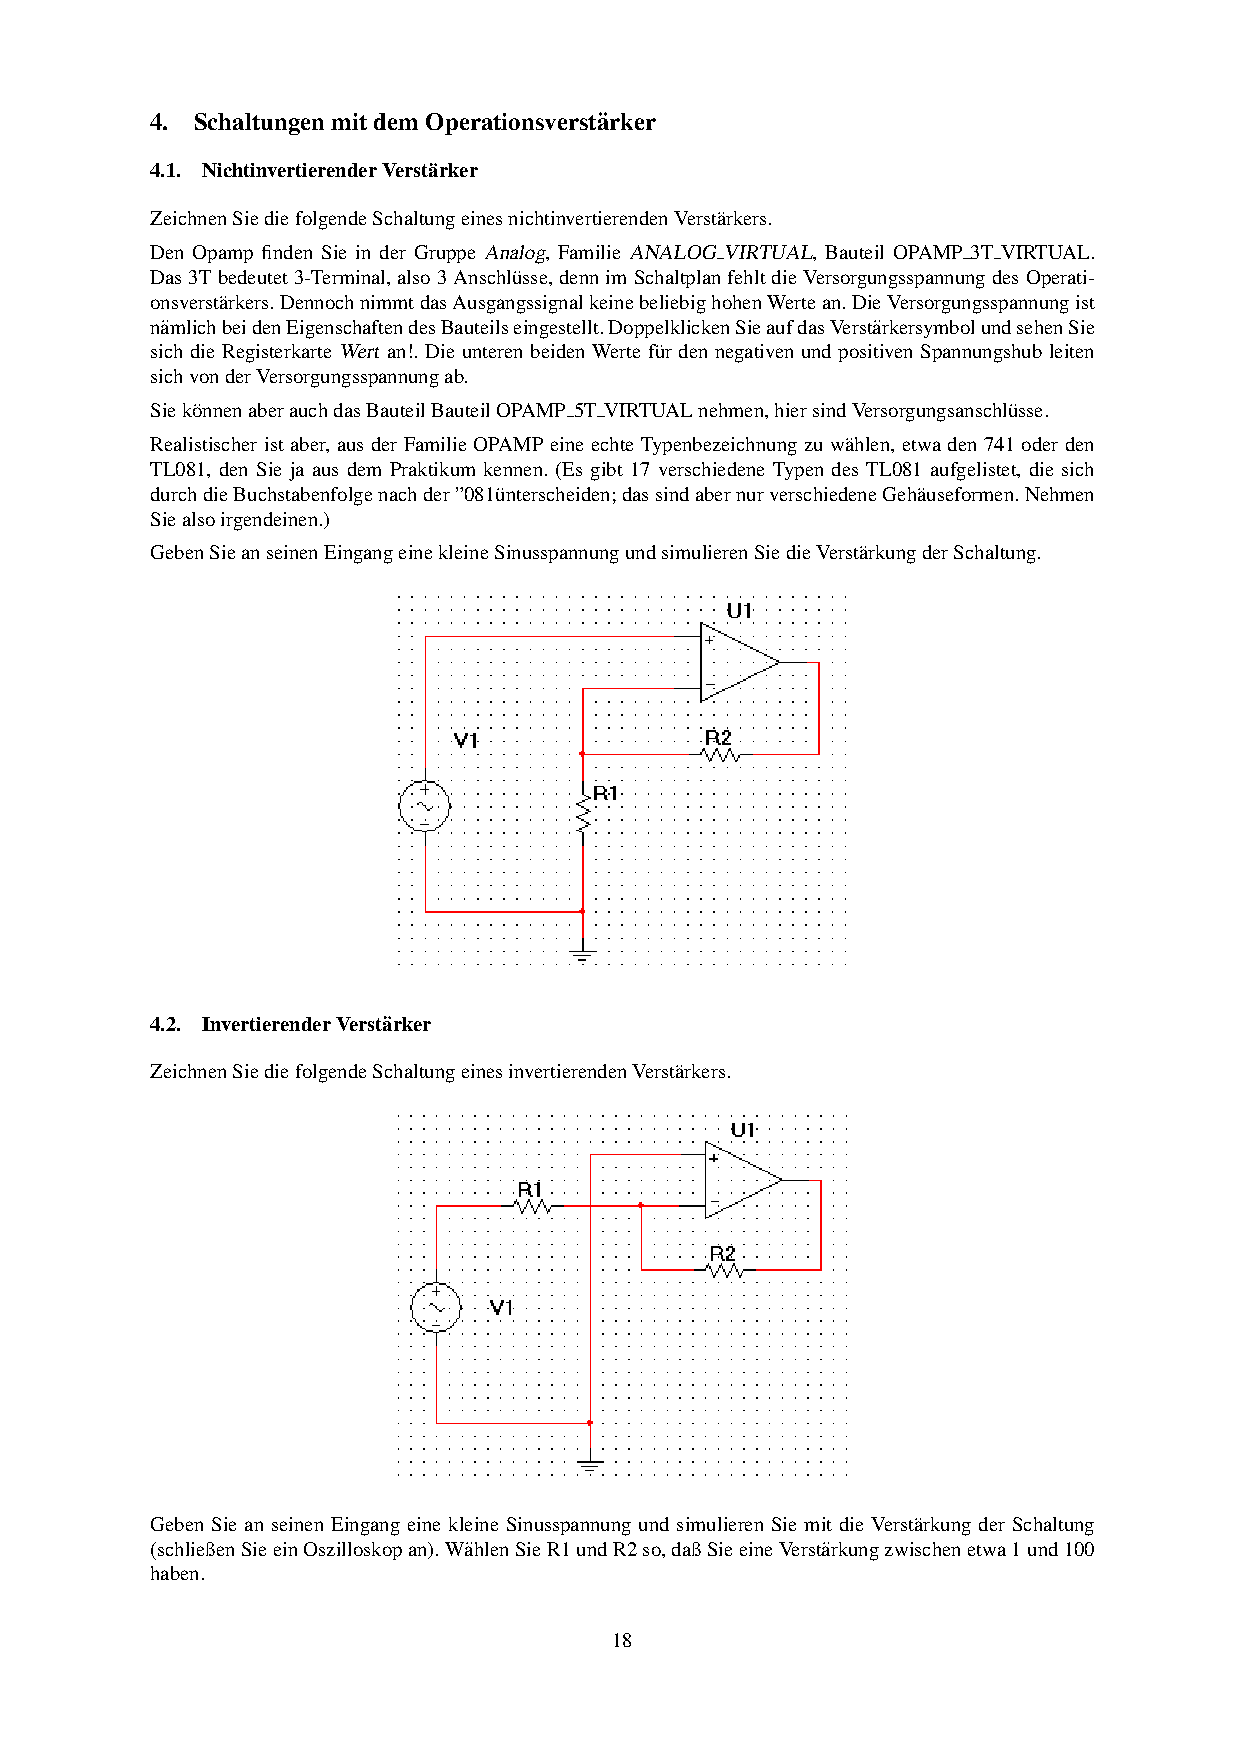
\includegraphics[trim = 10mm 130mm 10mm 100mm, clip, scale = 1]{ep5_14[Page18].pdf}
  	\caption[Schaltskizze für einen nicht invertierenden Verstärker]{Schaltskizze für einen nicht invertierenden Verstärker\footnotemark}
  \label{fig:4_a_1}
\end{figure}
\footnotetext{Abbildung entnommen von http://www.atlas.uni-wuppertal.de/$\sim$kind/ep5\_14.pdf Seite 18 am 22.11.2014}

\subsubsection{Versuchsdurchführung}
%erklären, !was! wir machen, !warum! wir das machen und mit welchem ziel
%(wichtig) präzize erklären, wie bei dem versuch vorgegangen und was gemacht wurde

Der Schaltplan wird nach Abbildung \ref{fig:4_a_1} aufgebaut und das Oszilloskop angeschlossen. Dann wird das Fenster des Oszilloskops geöffnet und die Simulation gestartet.


\subsubsection{Auswertung}
%zuerst !alle! errechneten werte entweder in ganzen sätzen aufzählen, oder in tabellen (übersichtlicher) dargestellen, sowie auf die verwendeten formeln verweisen (die referenzierung der formel kann in der überschrift stehen)
%kurz erwähnen (vor der tabelle), warum wir das ganze ausrechnen bzw. was wir dort ausrechnen
%danach histogramme und plots erstellen, wobei wenn möglich funktionen durch die plots gelegt werden (zur not können auch splines benutzt werden, was aber angegeben werden muss)
%bei fits immer die funktion und das reduzierte chiquadrat mit angegeben, wobei auf verständlichkeit beim entziffern der zehnerpotenzen geachtet werden muss z.b. f(x)=(wert+-fehler)\cdot10^{irgendeine zahl}\cdot x + (wert+-fehler)\cdot10^{irgendeine zahl}
%bei jedem fit erklären, nach welchem zusammenhang gefittet wurde und warum!
%bei plots darauf achten, dass die achsenbeschriftung (auch die tics) die richtige größe haben und die legende im plot nicht die messwerte verdeckt
%kurz die aufgabenstellung abhandeln
%2-----------------------------------------------2

Es sollte die Verstärkung des Ausgangssignals gemessen werden, dabei wurde einer Verstärkung von 101 erwartet. In Abbildung \ref{fig:4_1_100} ist zu erkenne, dass die Verstärkung mindestens 100 beträgt. In Abbildung \ref{fig:4_1_101} wurden die Verschiebungen entfernt und ein kleinerer Ausschnitt betrachtet, es lässt sich erkennen, dass die Ausgangskurve (blau) ca. eine Einheit über der Eingangskurve (rot) liegt.

\begin{figure}[H]
        \centering
        \begin{subfigure}[b]{0.48\textwidth}
               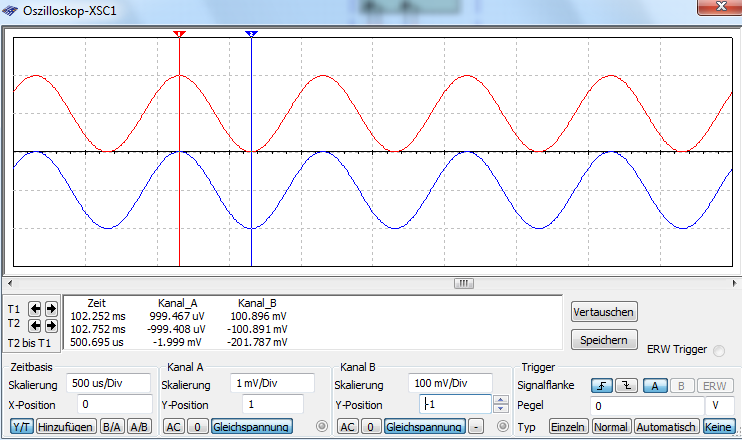
\includegraphics[scale = 0.4]{4_1_100.PNG}
				\caption[Aufnahme der Verstärkung]{Aufnahme der Verstärkung\footnotemark}
 				 \label{fig:4_1_100}
        \end{subfigure}%
        %~ %add desired spacing between images, e. g. ~, \quad, \qquad, \hfill etc.
          %(or a blank line to force the subfigure onto a new line)
        \hfill
        \begin{subfigure}[b]{0.48\textwidth}
                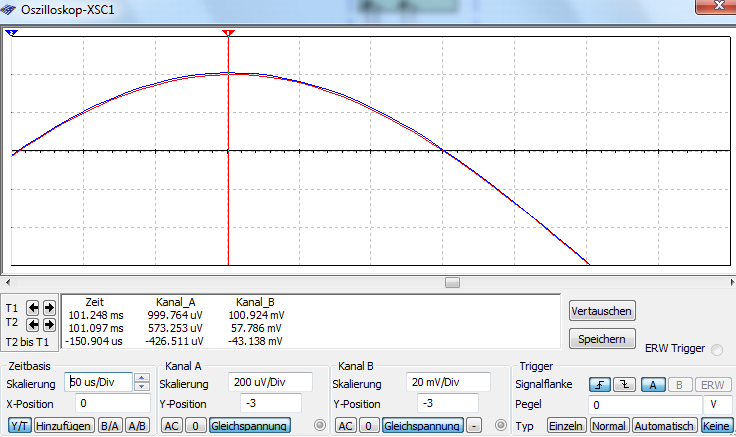
\includegraphics[scale = 0.4]{4_1_101.PNG}
  				\caption[Nahaufnahme der Verstärkung]{Nahaufnahme der Verstärkung\footnotemark}
  				\label{fig:4_1_101}
        \end{subfigure}
        \caption{Zwei Aufnahmen der Verstärkung}
        \label{fig:4_1}
\end{figure}

\subsubsection{Diskussion}
%(immer) die gemessenen werte und die bestimmten werte über die messfehler mit literaturwerten oder untereinander vergleichen
%in welchem fehlerintervall des messwertes liegt der literaturwert oder der vergleichswert?
%wie ist der relative anteil des fehlers am messwert und damit die qualität unserer messung?
%in einem satz erklären, wie gut unser fehler und damit unsere messung ist
%kurz erläutern, wie systematische fehler unsere messung beeinflusst haben könnten
%(wichtig) zum schluss ansprechen, in wie weit die ergebnisse mit der theoretischen vorhersage übereinstimmen
%--------------------------------------------------------------------------------------------
%falls tabellen mit den messwerten zu lang werden, kann die section mit den messwerten auch hinter der diskussion angefügt bzw. eine section mit dem anhang eingefügt werden.
%1-----------------------------------------------1

Wie erwartet ergab die Simulation eine Verstärkung um den Faktor 101.





\subsection{Invertierender Verstärker}
%kurz das ziel dieses versuchsteiles ansprechen, damit keine zwei überschriften direkt übereinander stehen!
%bei schwierigeren versuchen kann auch der theoretische hintergrund erläutert werden. (mit formeln, herleitungen und erklärungen)
\subsubsection{Verwendete Geräte}
%(immer) eine skizze oder ein foto einfügen, die geräte/materialien !nummerieren! und z.b. eine legende dazu schreiben, besser wäre es das ganze in einem Fließtext gut zu beschreiben.
%falls am anfang des versuches nicht klar ist, was alles verwendet wird, wenn möglich erst am ende ein großes foto von den verwendeten materialien machen!\\

Es werden ein Funktionsgenerator, ein Widerstand, ein Kondensator und ein Op-Amp verwendet.

\subsubsection{Verwendete Formeln}
%eine legende kann angefertigt werden, die selbstverständlichen buchstaben müssen nicht extra erklärt werden
%mit knappen erklärungen die !verwendeten! formeln, sowie die zugehörige fehlerrechnung einfügen
%2-----------------------------------------------2
%ab hier kann nochmal in einzelne versuchsteile unterteilt werden
\subsubsection{Versuchsaufbau}
%skizze zum versuchsaufbau (oder foto) einfügen,   es muss erklärt werden wie das ganze funktioniert und welche speziellen einstellungen verwendet wurden (z.b. welche knöpfe an den geräten für die messung verdreht wurden)

R1 ist ein 10k$\Omega$ und R2 ein 100$\Omega$ Widerstand. Die Sinusamplitude wurde mit 1mV angelegt.

\begin{figure}[H] 
  \centering
    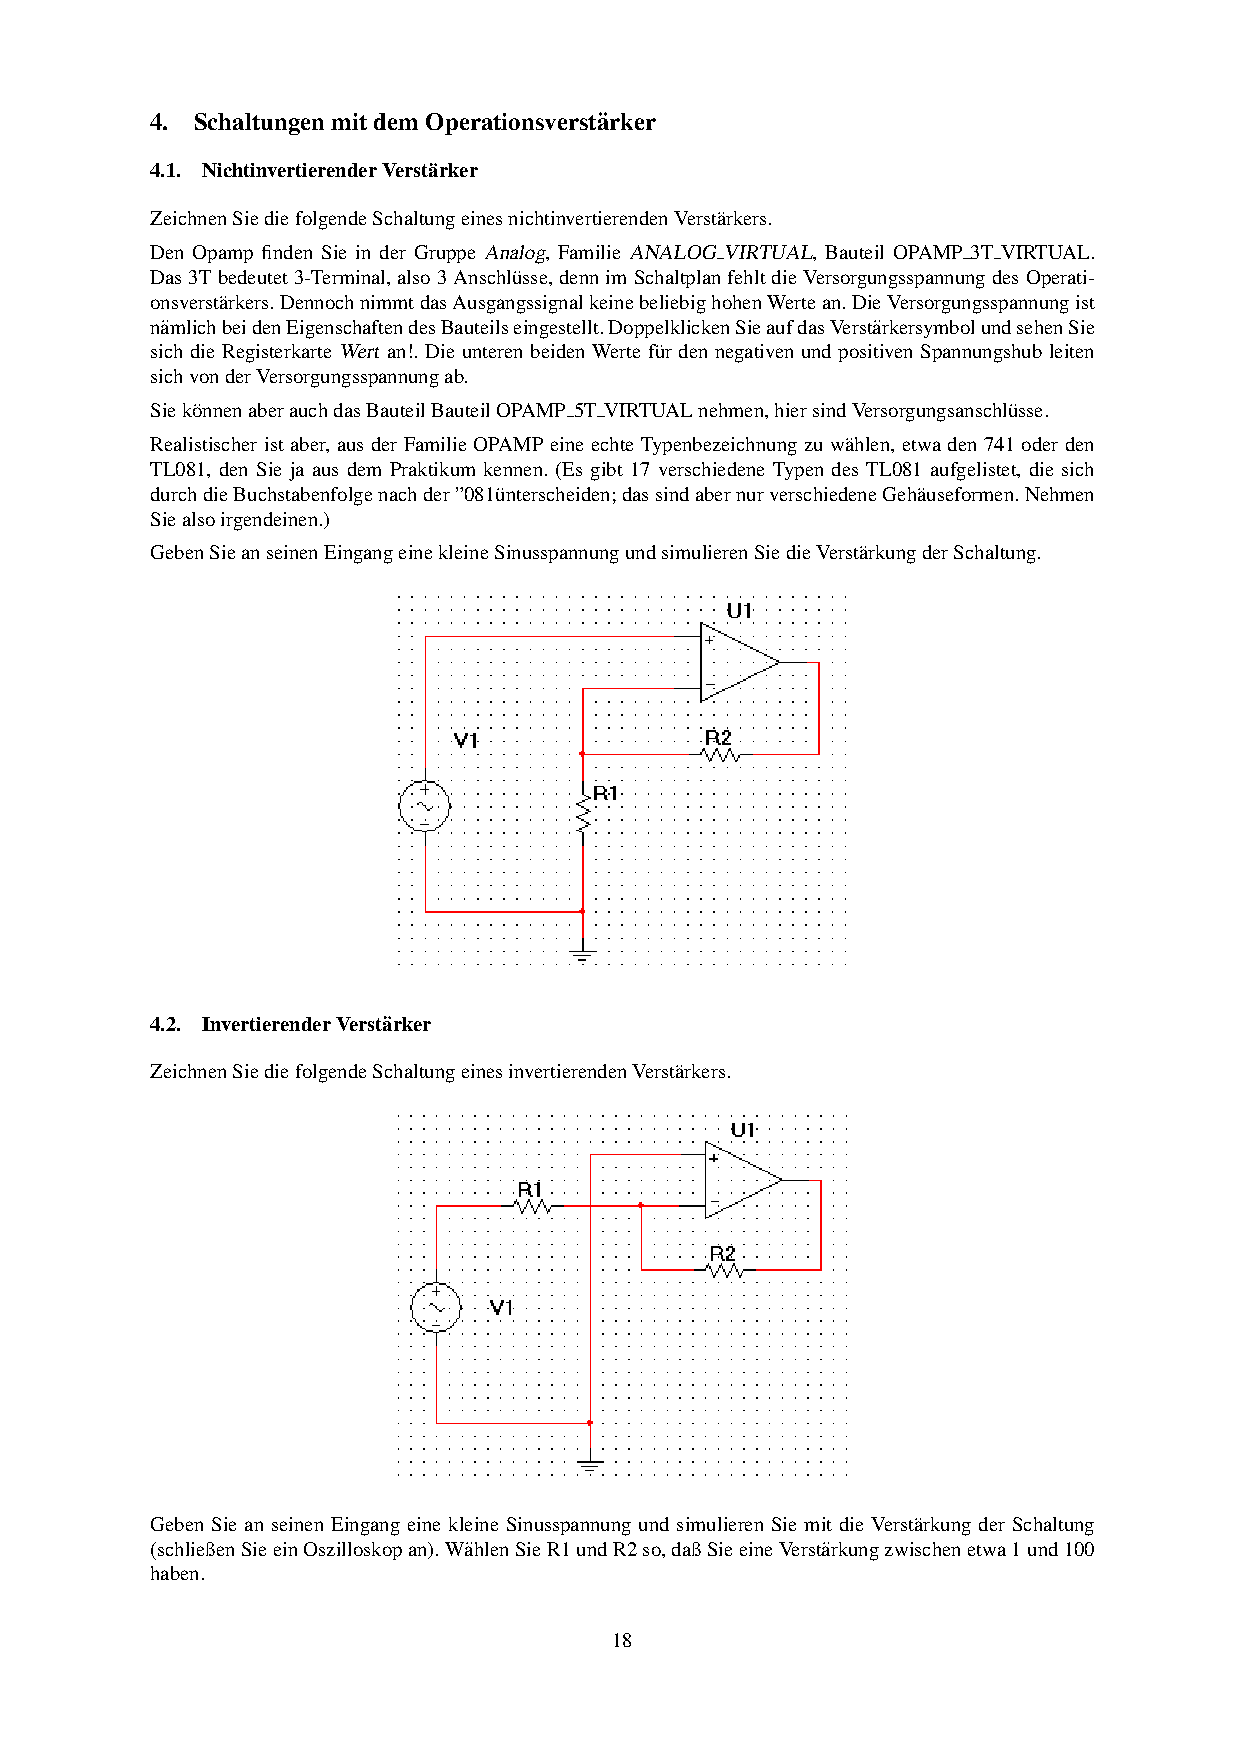
\includegraphics[trim = 10mm 45mm 10mm 190mm, clip, scale = 1]{ep5_14[Page18].pdf}
  	\caption[Schaltskizze für einen Invertierender Verstärker]{Schaltskizze für einen Invertierender Verstärker\footnotemark}
  \label{fig:4_a_2}
\end{figure}
\footnotetext{Abbildung entnommen von http://www.atlas.uni-wuppertal.de/$\sim$kind/ep5\_14.pdf Seite 18 am 22.11.2014}

\subsubsection{Versuchsdurchführung}
%erklären, !was! wir machen, !warum! wir das machen und mit welchem ziel
%(wichtig) präzize erklären, wie bei dem versuch vorgegangen und was gemacht wurde

Es wir die Schaltung nach Abbildung \ref{fig:4_a_2} aufgebaut und das Oszilloskop angeschlossen. Dann wird das Fenster des Oszilloskops aufgerufen und die Simulation gestartet. 

\subsubsection{Auswertung}
%zuerst !alle! errechneten werte entweder in ganzen sätzen aufzählen, oder in tabellen (übersichtlicher) dargestellen, sowie auf die verwendeten formeln verweisen (die referenzierung der formel kann in der überschrift stehen)
%kurz erwähnen (vor der tabelle), warum wir das ganze ausrechnen bzw. was wir dort ausrechnen
%danach histogramme und plots erstellen, wobei wenn möglich funktionen durch die plots gelegt werden (zur not können auch splines benutzt werden, was aber angegeben werden muss)
%bei fits immer die funktion und das reduzierte chiquadrat mit angegeben, wobei auf verständlichkeit beim entziffern der zehnerpotenzen geachtet werden muss z.b. f(x)=(wert+-fehler)\cdot10^{irgendeine zahl}\cdot x + (wert+-fehler)\cdot10^{irgendeine zahl}
%bei jedem fit erklären, nach welchem zusammenhang gefittet wurde und warum!
%bei plots darauf achten, dass die achsenbeschriftung (auch die tics) die richtige größe haben und die legende im plot nicht die messwerte verdeckt
%kurz die aufgabenstellung abhandeln
%2-----------------------------------------------2

Es wurde eine Phasenverschiebung von 180 Grad und eine Verstärkung von 100 erwartet, was in Abbildung \ref{fig:4_2} zu sehen ist. Es ist zu beachten, dass in der Abbildung \ref{fig:4_2} die beiden Kurven jeweils verschoben wurden.

\begin{figure}[H] 
  \centering
    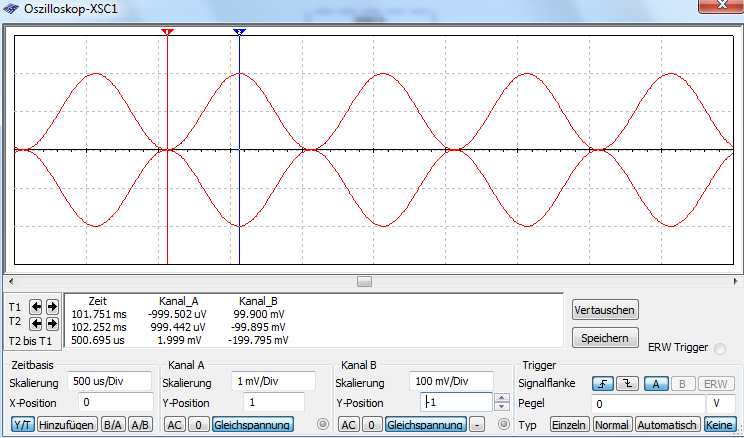
\includegraphics[ scale = 0.7]{4_2.PNG}
  	\caption[Aufnahme des Oszilloskops]{Aufnahme des Oszilloskops}
  \label{fig:4_2}
\end{figure}



\subsubsection{Diskussion}
%(immer) die gemessenen werte und die bestimmten werte über die messfehler mit literaturwerten oder untereinander vergleichen
%in welchem fehlerintervall des messwertes liegt der literaturwert oder der vergleichswert?
%wie ist der relative anteil des fehlers am messwert und damit die qualität unserer messung?
%in einem satz erklären, wie gut unser fehler und damit unsere messung ist
%kurz erläutern, wie systematische fehler unsere messung beeinflusst haben könnten
%(wichtig) zum schluss ansprechen, in wie weit die ergebnisse mit der theoretischen vorhersage übereinstimmen
%--------------------------------------------------------------------------------------------
%falls tabellen mit den messwerten zu lang werden, kann die section mit den messwerten auch hinter der diskussion angefügt bzw. eine section mit dem anhang eingefügt werden.
%1-----------------------------------------------1

Wie erwartet wurde eine Verstärkung von 100 gemessen und das Signal invertiert ausgegeben.


\subsection{Differenzierer}
%kurz das ziel dieses versuchsteiles ansprechen, damit keine zwei überschriften direkt übereinander stehen!
%bei schwierigeren versuchen kann auch der theoretische hintergrund erläutert werden. (mit formeln, herleitungen und erklärungen)

In diesem Versuchsteil soll der Differenzierer simuliert werden. Mit einem Differenzierer wird die Ableitung des Eingangssignals ausgegeben.

\subsubsection{Verwendete Geräte}
%(immer) eine skizze oder ein foto einfügen, die geräte/materialien !nummerieren! und z.b. eine legende dazu schreiben, besser wäre es das ganze in einem Fließtext gut zu beschreiben.
%falls am anfang des versuches nicht klar ist, was alles verwendet wird, wenn möglich erst am ende ein großes foto von den verwendeten materialien machen!\\

Es werden ein Funktionsgenerator, ein Widerstand, ein Kondensator und ein Op-Amp verwendet.


\subsubsection{Versuchsaufbau}
%skizze zum versuchsaufbau (oder foto) einfügen,   es muss erklärt werden wie das ganze funktioniert und welche speziellen einstellungen verwendet wurden (z.b. welche knöpfe an den geräten für die messung verdreht wurden)

C1 ist ein 100$\mu$F Kondensator, R1 ein 1k$\Omega$ Widerstand und V1 ein Sinusgenerator der mit 10mV und 100Hz betrieben wird.

\begin{figure}[H] 
  \centering
    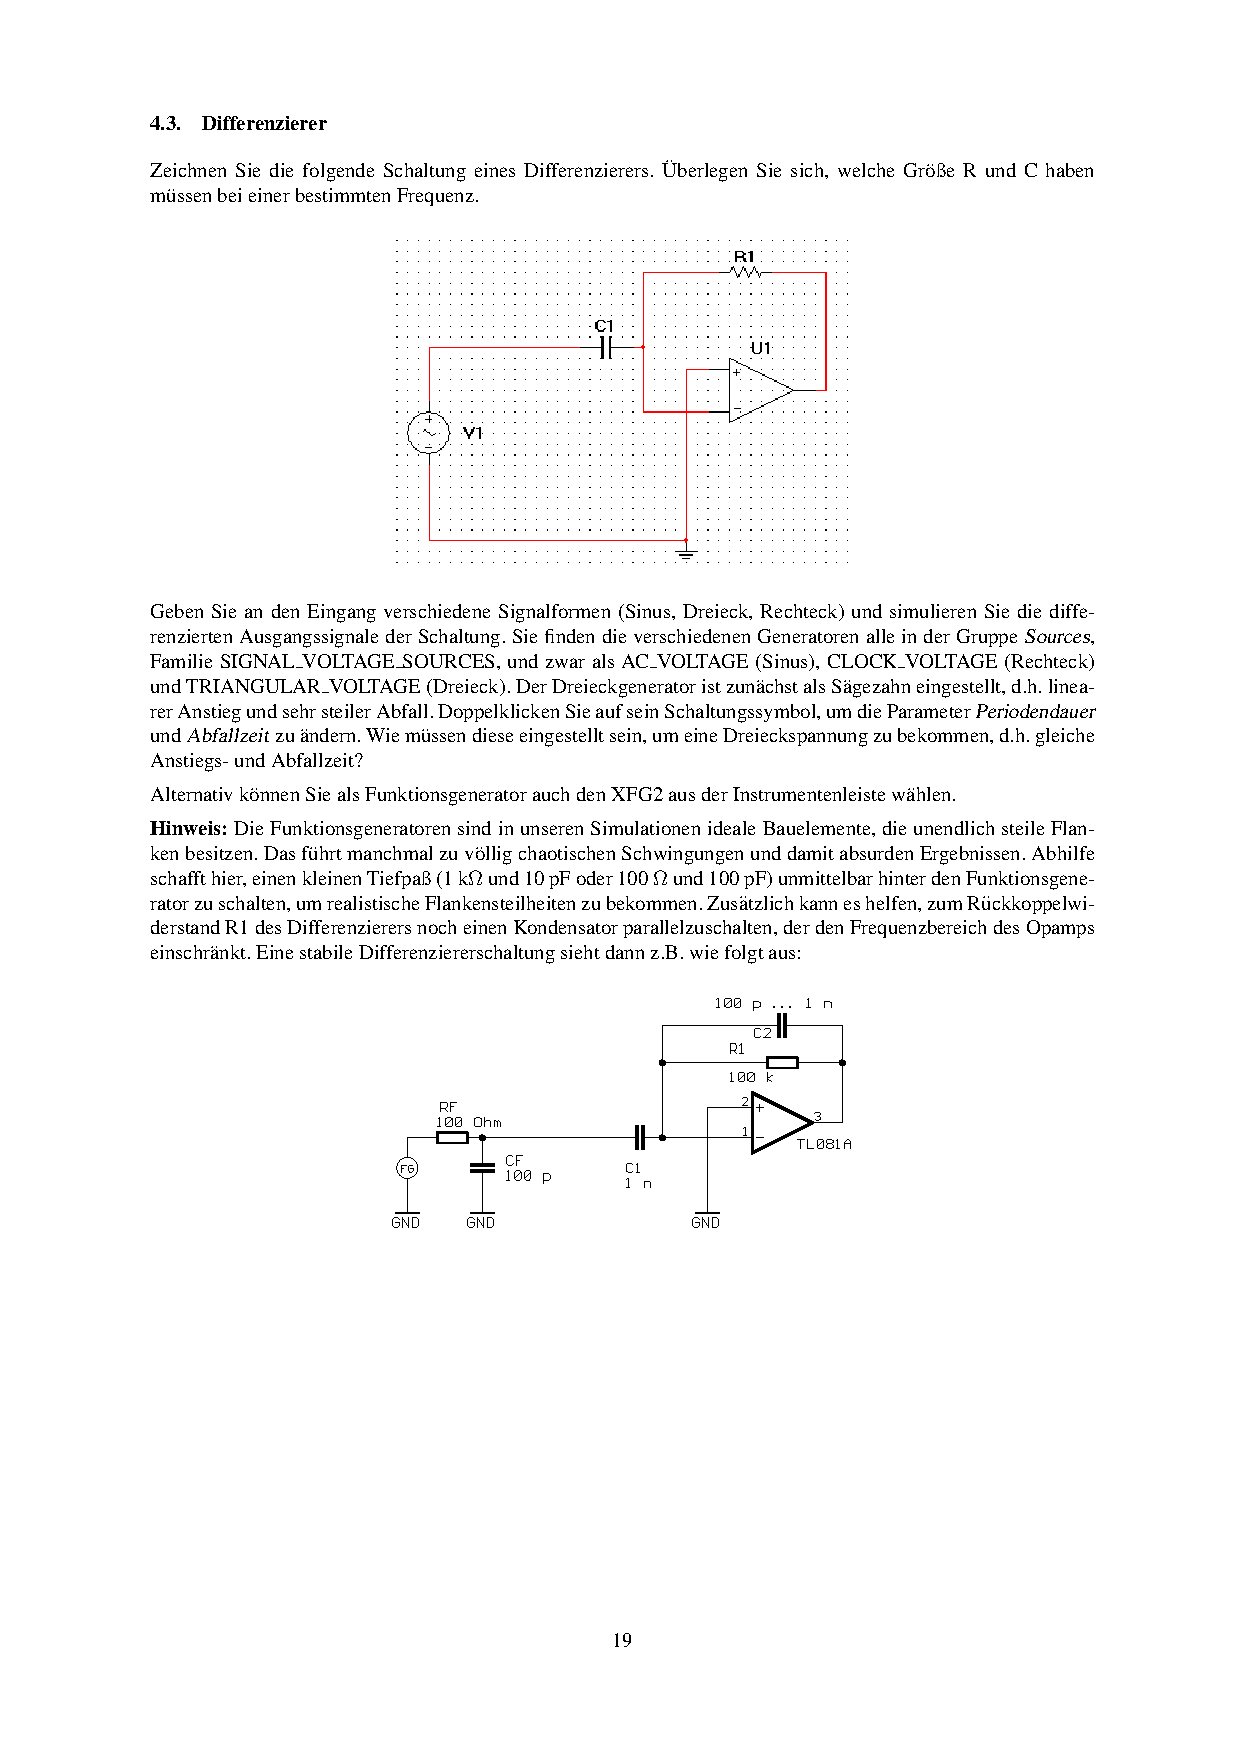
\includegraphics[trim = 10mm 200mm 10mm 40mm, clip, scale = 1]{ep5_14[Page19].pdf}
  	\caption[Schaltskizze für einen Differenzierer]{Schaltskizze für einen Differenzierer\footnotemark}
  \label{fig:4_a_3}
\end{figure}
\footnotetext{Abbildung entnommen von http://www.atlas.uni-wuppertal.de/$\sim$kind/ep5\_14.pdf Seite 19 am 22.11.2014}

\subsubsection{Versuchsdurchführung}
%erklären, !was! wir machen, !warum! wir das machen und mit welchem ziel
%(wichtig) präzize erklären, wie bei dem versuch vorgegangen und was gemacht wurde

Die Schaltung wird nach Abbildung \ref{fig:4_a_3} aufgebaut, dabei wird noch der Typ der Eingangsfrequenz ausgewählt und das Oszilloskop angeschlossen. Dann wird das Fenster des Oszilloskops geöffnet und die Simulation gestartet. Die Kurve auf dem Oszilloskop aufgenommen.

\subsubsection{Auswertung}
%zuerst !alle! errechneten werte entweder in ganzen sätzen aufzählen, oder in tabellen (übersichtlicher) dargestellen, sowie auf die verwendeten formeln verweisen (die referenzierung der formel kann in der überschrift stehen)
%kurz erwähnen (vor der tabelle), warum wir das ganze ausrechnen bzw. was wir dort ausrechnen
%danach histogramme und plots erstellen, wobei wenn möglich funktionen durch die plots gelegt werden (zur not können auch splines benutzt werden, was aber angegeben werden muss)
%bei fits immer die funktion und das reduzierte chiquadrat mit angegeben, wobei auf verständlichkeit beim entziffern der zehnerpotenzen geachtet werden muss z.b. f(x)=(wert+-fehler)\cdot10^{irgendeine zahl}\cdot x + (wert+-fehler)\cdot10^{irgendeine zahl}
%bei jedem fit erklären, nach welchem zusammenhang gefittet wurde und warum!
%bei plots darauf achten, dass die achsenbeschriftung (auch die tics) die richtige größe haben und die legende im plot nicht die messwerte verdeckt
%kurz die aufgabenstellung abhandeln
%2-----------------------------------------------2

In Abbildung \ref{fig:4_3} sind die Eingangs- und Ausgangssignale für Rechteck- (Abbildung \ref{fig:4_3_recht}), Dreieck- (Abbildung \ref{fig:4_3_drei}) und Sinusspannung (Abbildung \ref{fig:4_3_sin}) zu sehen. Alle Eingangssignale wurden korrekt differenziert.

\begin{figure}[H]
        \centering
        \begin{subfigure}[t]{0.28\textwidth}
                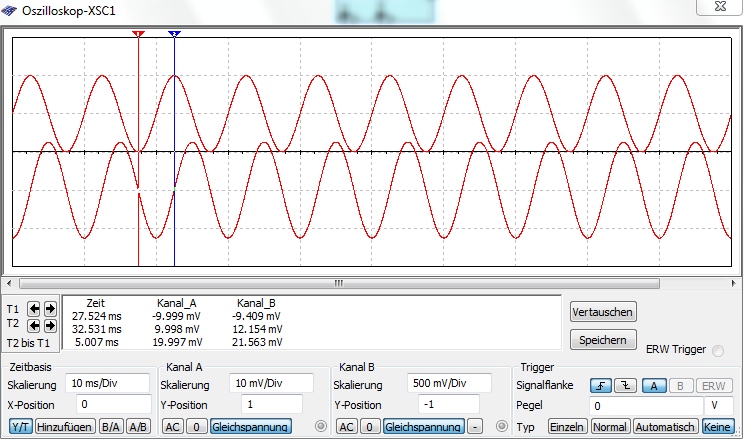
\includegraphics[width=\textwidth , scale = 0.4]{4_3_sin.PNG}
                \caption[Aufnahme des Sinussignals]{Aufnahme des Sinussignals}
                \label{fig:4_3_sin}
        \end{subfigure}%
       % ~ %add desired spacing between images, e. g. ~, \quad, \qquad, \hfill etc.
          %(or a blank line to force the subfigure onto a new line)
        \hfill
        \begin{subfigure}[t]{0.28\textwidth}
                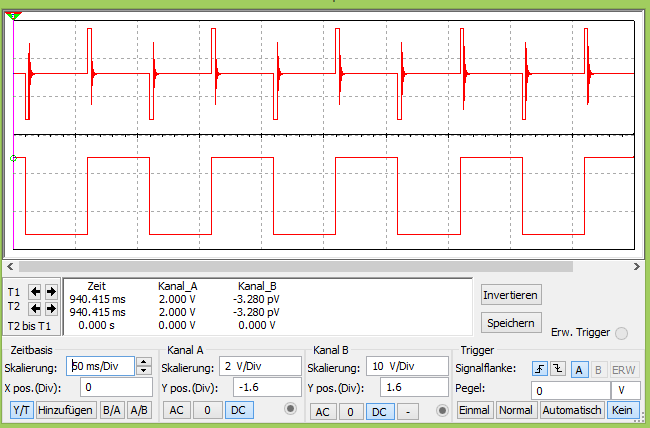
\includegraphics[width=\textwidth , scale = 0.4]{4_3_recht.PNG}
                \caption[Aufnahme des Rechtecksignals]{Aufnahme des Rechtecksignals}
                \label{fig:4_3_recht}
        \end{subfigure}
       % ~ %add desired spacing between images, e. g. ~, \quad, \qquad, \hfill etc.
          %(or a blank line to force the subfigure onto a new line)
        \hfill
        \begin{subfigure}[t]{0.28\textwidth}
                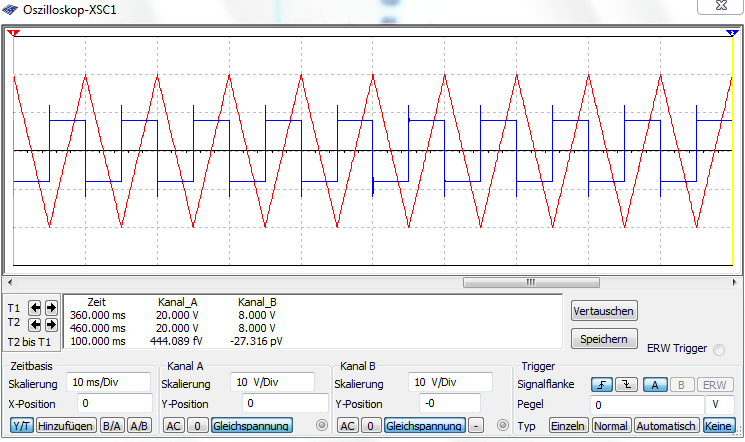
\includegraphics[width=\textwidth , scale = 0.4]{4_3_drei.PNG}
                \caption[Aufnahme des Dreiecksignals]{Aufnahme des Dreiecksignals}
  				\label{fig:4_3_drei}
        \end{subfigure}
        \caption{Kurven  für Rechteck-, Dreieck- und Sinussignal}
        \label{fig:4_3}
\end{figure}

\subsubsection{Diskussion}
%(immer) die gemessenen werte und die bestimmten werte über die messfehler mit literaturwerten oder untereinander vergleichen
%in welchem fehlerintervall des messwertes liegt der literaturwert oder der vergleichswert?
%wie ist der relative anteil des fehlers am messwert und damit die qualität unserer messung?
%in einem satz erklären, wie gut unser fehler und damit unsere messung ist
%kurz erläutern, wie systematische fehler unsere messung beeinflusst haben könnten
%(wichtig) zum schluss ansprechen, in wie weit die ergebnisse mit der theoretischen vorhersage übereinstimmen
%--------------------------------------------------------------------------------------------
%falls tabellen mit den messwerten zu lang werden, kann die section mit den messwerten auch hinter der diskussion angefügt bzw. eine section mit dem anhang eingefügt werden.
%1-----------------------------------------------1

Die Simulation des Differenzieres hat wie erwarte funktioniert.

\subsection{Integrierer}
%kurz das ziel dieses versuchsteiles ansprechen, damit keine zwei überschriften direkt übereinander stehen!
%bei schwierigeren versuchen kann auch der theoretische hintergrund erläutert werden. (mit formeln, herleitungen und erklärungen)

In diesem Versuchsteil sollte die Schaltung eines Integrierers simuliert werden. Ein Integrierer gibt die Integration des Eingangssignals aus.

\subsubsection{Verwendete Geräte}
%(immer) eine skizze oder ein foto einfügen, die geräte/materialien !nummerieren! und z.b. eine legende dazu schreiben, besser wäre es das ganze in einem Fließtext gut zu beschreiben.
%falls am anfang des versuches nicht klar ist, was alles verwendet wird, wenn möglich erst am ende ein großes foto von den verwendeten materialien machen!\\

Es werden ein Funktionsgenerator, ein Widerstand, ein Kondensator und ein Op-Amp verwendet.


\subsubsection{Versuchsaufbau}
%skizze zum versuchsaufbau (oder foto) einfügen,   es muss erklärt werden wie das ganze funktioniert und welche speziellen einstellungen verwendet wurden (z.b. welche knöpfe an den geräten für die messung verdreht wurden)

R1 ist ein 1k$\Omega$ Widerstand, C1 ein 1$\mu$F Kondensator und V1 ein Funktionsgenerator.

\begin{figure}[H] 
  \centering
    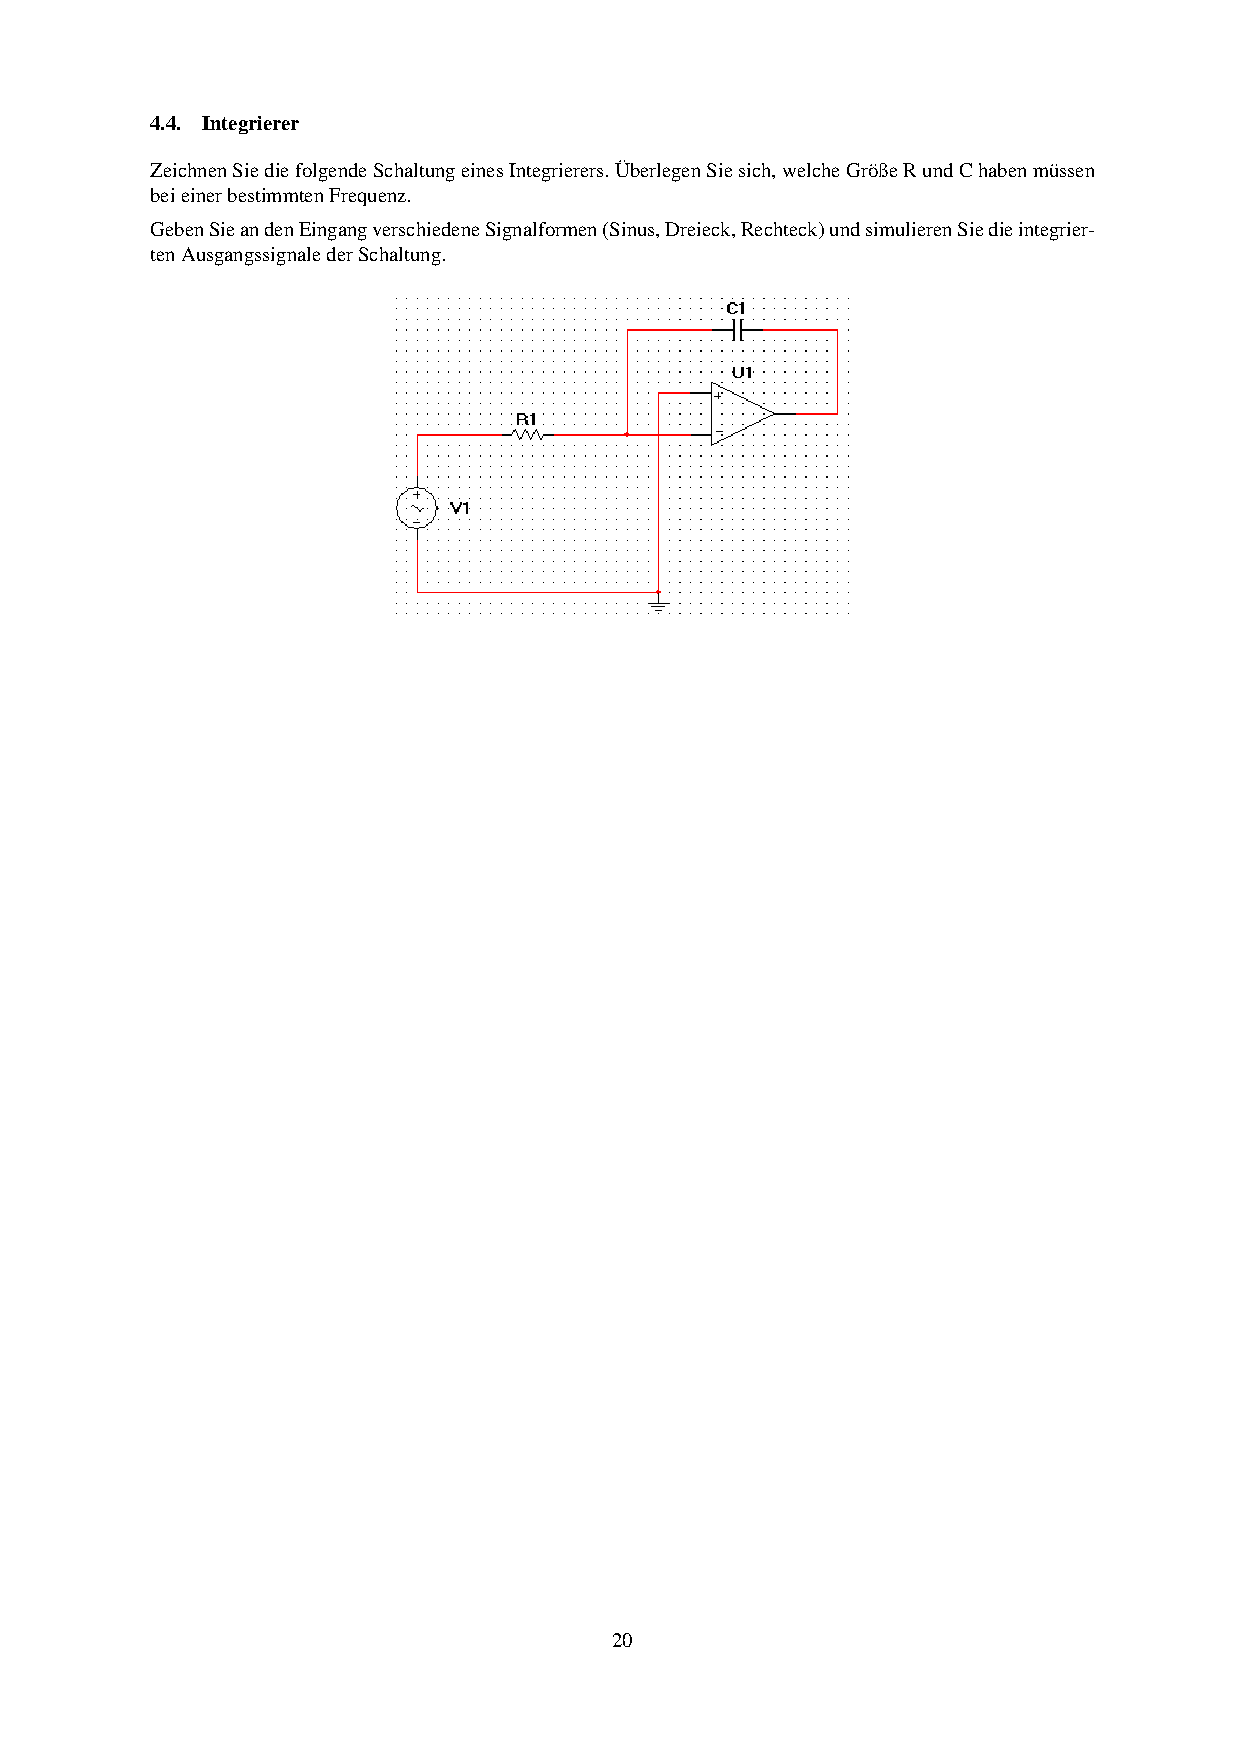
\includegraphics[trim = 10mm 180mm 10mm 50mm, clip, scale = 1]{ep5_14[Page20].pdf}
  	\caption[Schaltskizze für einen Integrierer]{Schaltskizze für einen Integrierer\footnotemark}
  \label{fig:4_a_4}
\end{figure}
\footnotetext{Abbildung entnommen von http://www.atlas.uni-wuppertal.de/$\sim$kind/ep5\_14.pdf Seite 20 am 22.11.2014}

\subsubsection{Versuchsdurchführung}
%erklären, !was! wir machen, !warum! wir das machen und mit welchem ziel
%(wichtig) präzize erklären, wie bei dem versuch vorgegangen und was gemacht wurde

Es wird die Schaltung nach Abbildung \ref{fig:4_a_4}, das Eingangssignal eingestellt und das Oszilloskop angeschlossen. Dann wird das Fenster des Oszilloskops aufgerufen und die Simulation gestartet. Die Kurve auf dem Oszilloskops wird dann aufgenommen.


\subsubsection{Auswertung}
%zuerst !alle! errechneten werte entweder in ganzen sätzen aufzählen, oder in tabellen (übersichtlicher) dargestellen, sowie auf die verwendeten formeln verweisen (die referenzierung der formel kann in der überschrift stehen)
%kurz erwähnen (vor der tabelle), warum wir das ganze ausrechnen bzw. was wir dort ausrechnen
%danach histogramme und plots erstellen, wobei wenn möglich funktionen durch die plots gelegt werden (zur not können auch splines benutzt werden, was aber angegeben werden muss)
%bei fits immer die funktion und das reduzierte chiquadrat mit angegeben, wobei auf verständlichkeit beim entziffern der zehnerpotenzen geachtet werden muss z.b. f(x)=(wert+-fehler)\cdot10^{irgendeine zahl}\cdot x + (wert+-fehler)\cdot10^{irgendeine zahl}
%bei jedem fit erklären, nach welchem zusammenhang gefittet wurde und warum!
%bei plots darauf achten, dass die achsenbeschriftung (auch die tics) die richtige größe haben und die legende im plot nicht die messwerte verdeckt
%kurz die aufgabenstellung abhandeln
%2-----------------------------------------------2

In Abbildung \ref{fig:4_4} sind die Eingangs- und Ausgangssignale für Rechteck- (Abbildung \ref{fig:4_4_recht}), Dreieck- (Abbildung \ref{fig:4_4_drei}) und Sinusspannung (Abbildung \ref{fig:4_4_sin}) zu sehen. Alle Eingangssignale wurden korrekt integriert.

\begin{figure}[H]
        \centering
        \begin{subfigure}[t]{0.28\textwidth}
                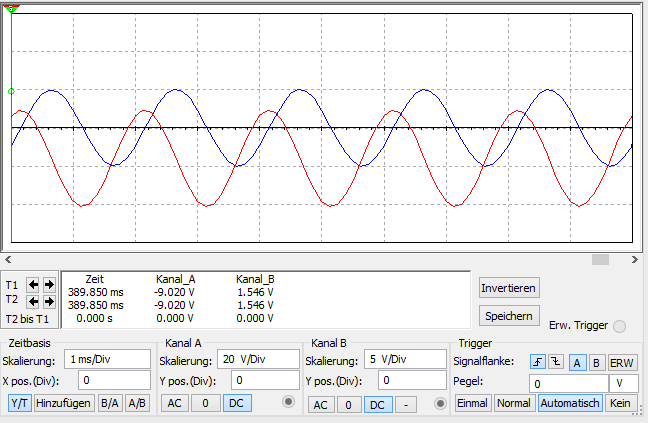
\includegraphics[width=\textwidth , scale = 0.4]{4_4_sin.PNG}
                \caption[Aufnahme des Sinussignals]{Aufnahme des Sinussignals}
                \label{fig:4_4_sin}
        \end{subfigure}%
       % ~ %add desired spacing between images, e. g. ~, \quad, \qquad, \hfill etc.
          %(or a blank line to force the subfigure onto a new line)
        \hfill
        \begin{subfigure}[t]{0.28\textwidth}
                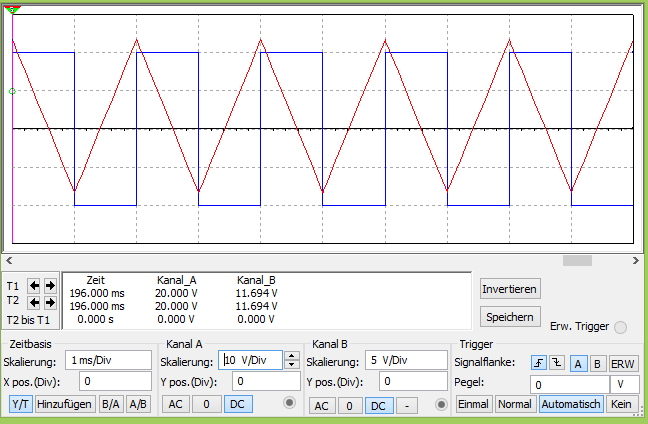
\includegraphics[width=\textwidth , scale = 0.4]{4_4_recht.PNG}
                \caption[Aufnahme des Rechtecksignals]{Aufnahme des Rechtecksignals}
                \label{fig:4_4_recht}
        \end{subfigure}
       % ~ %add desired spacing between images, e. g. ~, \quad, \qquad, \hfill etc.
          %(or a blank line to force the subfigure onto a new line)
        \hfill
        \begin{subfigure}[t]{0.28\textwidth}
                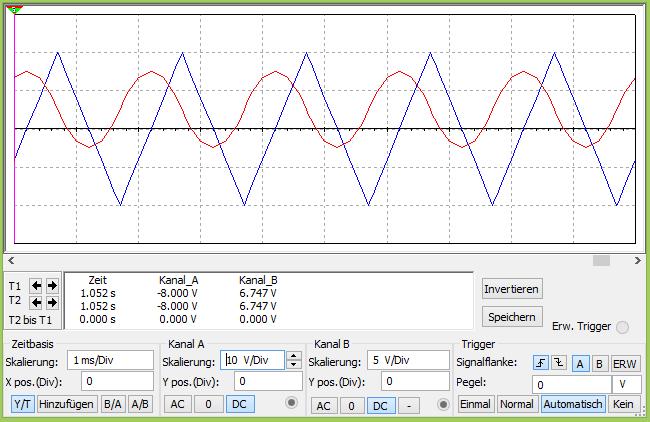
\includegraphics[width=\textwidth , scale = 0.4]{4_4_drei.PNG}
                \caption[Aufnahme des Dreiecksignals]{Aufnahme des Dreiecksignals}
  				\label{fig:4_4_drei}
        \end{subfigure}
        \caption{Kurven  für Rechteck-, Dreieck- und Sinussignal}
        \label{fig:4_4}
\end{figure}

\subsubsection{Diskussion}
%(immer) die gemessenen werte und die bestimmten werte über die messfehler mit literaturwerten oder untereinander vergleichen
%in welchem fehlerintervall des messwertes liegt der literaturwert oder der vergleichswert?
%wie ist der relative anteil des fehlers am messwert und damit die qualität unserer messung?
%in einem satz erklären, wie gut unser fehler und damit unsere messung ist
%kurz erläutern, wie systematische fehler unsere messung beeinflusst haben könnten
%(wichtig) zum schluss ansprechen, in wie weit die ergebnisse mit der theoretischen vorhersage übereinstimmen
%--------------------------------------------------------------------------------------------
%falls tabellen mit den messwerten zu lang werden, kann die section mit den messwerten auch hinter der diskussion angefügt bzw. eine section mit dem anhang eingefügt werden.
%1-----------------------------------------------1

Die Simulation des Integrierers hat wie erwarte funktioniert.

\section{Fazit}
%im fazit nochmal alles zusammenfassen und den verlauf der messung abschätzen
%gravierende sytematische probleme bei den messungen nochmal betonen und die wertigkeit unserer ergebnisse einordnen

In diesem Versuch haben wir verschiedene Schaltungen, welche wir zuvor schon in echt untersucht hatten simuliert. Dabei zeigte sich das Multisim bei allen Schaltungen die zuvor bestimmten Messungen qualitativ reproduzieren konnte. Multisim eignet sich sehr gut, um Schaltungen zu Simulieren und ihr Verhalten zu untersuchen, dabei sollte man jedoch beachten, das Multisim nicht die Zerstörung von Bauteilen mit Simuliert, bei zu hohen Strömen bzw. Spannungen.

\end{document}

